\documentclass[preprint,12pt]{elsarticle}
\usepackage[T1]{fontenc}
\usepackage{lmodern}
\usepackage{amsmath,amssymb,amsthm}
\usepackage{booktabs}
\usepackage{graphicx}
\usepackage{tikz}
\usetikzlibrary{calc}
\usepackage[hidelinks]{hyperref}
\usepackage{xcolor}

\newcommand{\R}{\mathbb{R}}
\newcommand{\bu}{\mathbf{u}}
\newcommand{\bv}{\mathbf{v}}
\newcommand{\bF}{\mathbf{F}}
\newcommand{\bn}{\mathbf{n}}
\newcommand{\rhat}{\hat{\mathbf{r}}}
\newcommand{\Pc}{\mathcal{P}}
\newcommand{\Pt}{\widetilde{\mathcal{P}}}
\newcommand{\Kc}{\mathcal{K}}
\newcommand{\Fc}{\mathcal{F}}
\newcommand{\jump}[1]{[\![#1]\!]}
\newcommand{\avg}[1]{\{\!\{#1\}\!\}}
\newcommand{\code}[1]{\texttt{#1}}
\newcommand{\curl}{\mathbf{curl}}
\newtheorem{theorem}{Theorem}
\newtheorem{proposition}{Proposition}
\newtheorem{lemma}{Lemma}
\theoremstyle{definition}
\newtheorem{definition}{Definition}
\newtheorem{remark}{Remark}

\journal{Journal of Computational Physics}

\begin{document}

\begin{frontmatter}
\title{Staggered kite finite elements with mass lumping for the shallow-water equations and the
compressible Euler equations on polygonal meshes}

\author{Oswald Knoth}

\begin{abstract}
Every polygonal mesh of the sphere or the plane --- triangles, quadrilaterals and the hexagons and
pentagons of Voronoi meshes --- is split into quadrilaterals (\emph{kites}) by joining the cell centres
with points on the edges. On the kite mesh we define a height space of tensor Gauss--Radau elements,
continuous inside every primal cell and broken across primal edges, and a velocity space of
Raviart--Thomas elements, normal-continuous inside every dual cell and broken across its boundary.
The height mass matrix is diagonal, the velocity mass matrix block diagonal with one block per dual
cell, and the discrete divergence and gradient are exact adjoints and free of the metric. The rotating
shallow-water scheme conserves mass and energy exactly and converges at second order on all mesh types.
For the pair $\mathrm{RT}_k\times Q_{k+1}$ we prove that the velocity space splits exactly into discrete
gradients and curls, at the price of one stationary height mode per primal cell.
The extension to the compressible Euler equations is a tensor product with a vertical $\mathrm{DG}_0\times
\mathrm{CG}_1$ discretization that is derived as a Galerkin method with the trapezoidal rule: the vertical
mass is diagonal, every Radau node carries an independent column, and the vertical energy exchange is
exact. Going from two to three dimensions exposes four problems that the shallow-water tests do not show:
a quadrature mismatch between the velocity mass and the projections, a consistency defect of the projected
transport of scalars, the instability of the vector-invariant momentum transport in flow faster than the
gravity waves --- which the higher vertical modes of a stratified atmosphere always are --- and the
different weighting of the sub-cell height modes by the horizontal and the vertical pressure gradient.
A discontinuous Galerkin transport of momentum, density and potential temperature removes the
instabilities. The model is quiet on a steady thermal wind, reproduces the linear growth rate of
baroclinic instability in an $f$-plane channel and gives the same baroclinic wave on hexagonal,
cubed-sphere and triangular meshes.
\end{abstract}

\begin{keyword}
staggered finite elements \sep mass lumping \sep dual cell method \sep polygonal meshes \sep
shallow-water equations \sep compressible Euler equations \sep HEVI
\end{keyword}
\end{frontmatter}

%==============================================================================
\section{Introduction}\label{sec:intro}

Compatible (mimetic) finite elements give the discrete operators of geophysical fluid dynamics the
structure of the continuous ones: the gradient is the negative adjoint of the divergence, the curl of a
gradient vanishes, and the semi-discrete equations conserve mass and energy
\cite{CotterShipton2012,McRaeCotter2014,NataleShiptonCotter2016}. Their extension to three dimensions
uses extruded elements whose vertical part is again a compatible pair \cite{NataleShiptonCotter2016,Melvin2019}.
The price is that the mass matrices of the usual pairs (e.g.\ $\mathrm{RT}_k\times\mathrm{DG}_k$) are not
diagonal, so an explicit step needs global solves. Finite-volume C grids \cite{Thuburn2009,Ringler2010,Zaengl2015}
avoid them with diagonal Hodge stars, at the price of first-order operators on general meshes.

Two families of methods obtain local mass matrices from staggered finite elements. Staggered
discontinuous Galerkin (SDG) methods \cite{ChungEngquist2006,ChungLamQian2015,DuChung2021} use two
staggered macro-element meshes, with one field continuous in the primal and the other in the dual macro
elements. Leng, Lan and Ju \cite{LengLanJu2026} built from them a conservative SDG method for the
shallow-water equations on the sphere: they split every polygon into triangles around an interior point,
take the velocity normal-continuous in the polygons and the height continuous in the pairs of triangles
around the edges, and prove mass and energy conservation, the absence of spurious pressure modes and a
steady geostrophic mode. The dual cell method of Wess, Kapidani, Codecasa and Sch\"oberl \cite{Wess2024}
splits the primal cells into quadrilaterals around the primal vertices and uses tensor-product spaces
whose degrees of freedom are quadrature points, so that the mass matrices are diagonal or block diagonal
to arbitrary order; they apply it to acoustic and electromagnetic waves.

This paper combines the two ideas for geophysical flows. The quadrilaterals of the dual cell method,
here called \emph{kites}, give tensor-product spaces with Gauss--Radau nodes and a diagonal height mass;
the Raviart--Thomas velocity of the SDG methods gives a mass flux with a block-diagonal mass and
exactly adjoint, metric-free operators. The heights are continuous in the primal cells and the velocity
in the dual cells, the opposite of \cite{LengLanJu2026}. The contributions are:
\begin{enumerate}
\item The kite spaces $H_p\times U_k\times Z_{k+1}$ on arbitrary polygonal meshes of the sphere with curved
  elements, their mass-lumped inner products and the metric-free divergence and gradient
  (Sections~\ref{sec:mesh}--\ref{sec:operators}).
\item For the default pair $U_1\times H_2$ an exact discrete Helmholtz decomposition of the velocity space
  and the characterization of its kernel: one stationary height mode per primal cell, given in closed form
  (Theorem~\ref{thm:kernel}).
\item An energy-conserving nonlinear shallow-water scheme with these spaces (Section~\ref{sec:sw}) and its
  validation on hexagonal, triangular and quadrilateral meshes (Section~\ref{sec:sw-results}).
\item A vertical discretization of the compressible Euler equations derived as a Galerkin method with the
  trapezoidal rule, with a diagonal vertical mass, independent columns at the Radau nodes and an exact
  vertical energy exchange, and its horizontally explicit, vertically implicit (HEVI) time discretization
  (Section~\ref{sec:3d}).
\item An analysis of what changes from two to three dimensions (Section~\ref{sec:2d3d}) and a
  discontinuous Galerkin (DG) transport that removes the resulting instabilities (Section~\ref{sec:dg}),
  validated on a thermal wind, a baroclinic channel and the baroclinic wave on the sphere
  (Section~\ref{sec:3d-results}).
\end{enumerate}
Section~\ref{sec:related} compares the method with the related ones; Section~\ref{sec:conclusions}
concludes.

%==============================================================================
\section{Kite meshes and mass-lumped inner products}\label{sec:mesh}

\subsection{Kite meshes}
Let $\Pc$ be a polygonal primal mesh of a closed surface $\Omega$ (the sphere of radius $a$ or a doubly
periodic plane) with $N$ cells, $E$ edges and $V$ vertices. Every cell $P\in\Pc$ with vertices
$w_1,\dots,w_n$ is split into $n$ kites
\[
  K_i = (w_i,\; m_i,\; c_P,\; m_{i-1}),\qquad i = 1,\dots,n,
\]
where $c_P$ is the cell centre and $m_i$ a point on the primal edge $(w_i,w_{i+1})$
(Figure~\ref{fig:kites}). The kites around a primal vertex $w$ form its dual cell $\widetilde P_w$, and
$\Kc$ denotes the set of all $2E$ kites. Every kite has the same local numbering: vertex~1 is the primal
vertex and vertex~3 the centre. Local edges~1 and~4 are halves of primal edges (\emph{primal faces});
local edges~2 and~3 join an edge point to the centre (\emph{dual faces}) and form the boundaries of the
dual cells. Every primal face is interior to a dual cell, every dual face interior to a primal cell.

\paragraph{Cell centres and edge points} The centre is the vertex of the orthogonal dual mesh when
there is one: the circumcentre of a triangle, the generator of a Voronoi cell. The generators of a Voronoi
mesh are recovered from the cells as the null vector of the homogeneous linear system
$g_i - g_j\parallel\bn_e$, $\bn_e\cdot(g_i+g_j) = 0$ over all edges $e$ between cells $i$ and $j$; for
the published MPAS and ICON meshes this reproduces the stored generators to $10^{-14}$. On other meshes
(cubed sphere, planes) the centre is the centroid. With an orthogonal dual, $m_i$ is the crossing of the
primal edge with the dual edge, so the dual faces lie on the dual edges; otherwise $m_i$ is the edge
midpoint.

\subsection{Reference map}
Every kite is the image of the reference square $\hat K = [-1,1]^2$ with the primal vertex at $(-1,-1)$
and the centre at $(1,1)$, so that the primal faces are $\{s = -1\}$ and $\{t = -1\}$ and the dual faces
$\{s = 1\}$ and $\{t = 1\}$. The map $F_K$ is the bilinear interpolant of the four vertices, on the sphere
followed by the radial projection $x\mapsto a\,x/|x|$ (curved elements). $J = DF_K$ is the $3\times2$
Jacobian and $\det J = |J_1\times J_2|$ the area element; the outward unit normal of the surface is
$\rhat = J_1\times J_2/|J_1\times J_2|$.

\subsection{Mass-lumped inner products}\label{sec:quadrature}
Let $r_0<\dots<r_p = 1$ be the $p+1$ Gauss--Radau points of $[-1,1]$ that include the end point $1$
(for $p = 0$ the single point $1$), with weights $\omega_0,\dots,\omega_p$. The tensor rule
$\{(r_a, r_b), \omega_a\omega_b\}$ on $\hat K$ integrates $Q_{2p}$ exactly. Its nodes lie inside the kite
($p^2$), on the two dual faces ($p$ each) and at the centre, never on a primal face. The lumped $L^2$
inner product of two scalar fields is
\begin{equation}\label{eq:lumped}
  (\eta,\phi)_h = \sum_{K\in\Kc}\sum_{a,b=0}^{p}\omega_a\omega_b\,\det J(r_a,r_b)\,\eta(F_K(r_a,r_b))\,
  \phi(F_K(r_a,r_b)).
\end{equation}
On flat kites $\det J$ is bilinear, so for $p\ge1$ the rule integrates $\det J$ times $Q_{2p-1}$ exactly
and the lumped mass of a constant is its exact mass. Velocity inner products and the nonlinear terms use a
Gauss rule of $(k+2)^2$ points per kite with precomputed metric terms.

\begin{figure}[t]
\centering
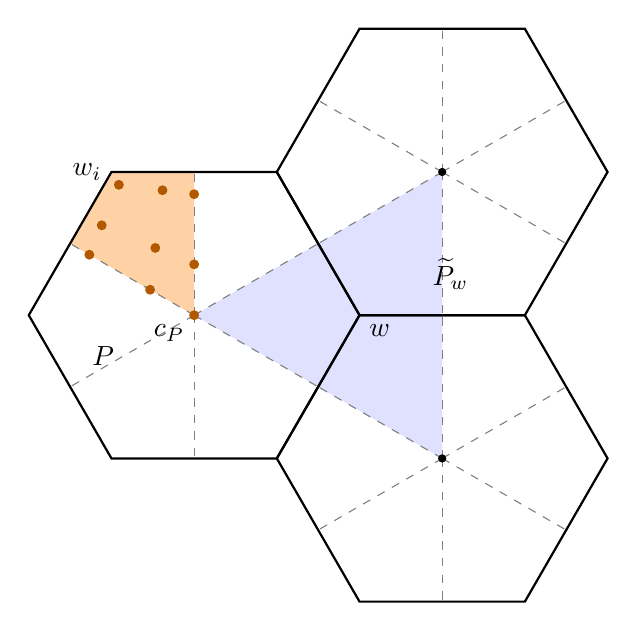
\begin{tikzpicture}[scale=2.1]
  \foreach \cx/\cy/\name in {0/0/P, 1.5/0.8660254/Q, 1.5/-0.8660254/R} {
    \coordinate (\name) at (\cx,\cy);
    \foreach \k in {0,...,5} {
      \coordinate (\name v\k) at ($(\cx,\cy)+({cos(60*\k)},{sin(60*\k)})$);
    }
  }
  \fill[blue!12] (Pv0) -- ($(Pv0)!0.5!(Pv1)$) -- (P) -- ($(Pv0)!0.5!(Pv5)$) -- cycle;
  \fill[blue!12] (Pv0) -- ($(Pv0)!0.5!(Pv1)$) -- (Q) -- ($(Pv0)!0.5!(Rv1)$) -- cycle;
  \fill[blue!12] (Pv0) -- ($(Pv0)!0.5!(Rv1)$) -- (R) -- ($(Pv0)!0.5!(Pv5)$) -- cycle;
  \fill[orange!35] (Pv2) -- ($(Pv2)!0.5!(Pv3)$) -- (P) -- ($(Pv2)!0.5!(Pv1)$) -- cycle;
  \foreach \name in {P,Q,R} {
    \draw[thick] (\name v0) -- (\name v1) -- (\name v2) -- (\name v3) -- (\name v4) -- (\name v5) -- cycle;
    \foreach \k [evaluate={\k as \kk using int(mod(\k+1,6))}] in {0,...,5} {
      \draw[gray, dashed] (\name) -- ($(\name v\k)!0.5!(\name v\kk)$);
    }
    \fill (\name) circle (0.025);
  }
  \coordinate (A) at (Pv2); \coordinate (B) at ($(Pv2)!0.5!(Pv3)$);
  \coordinate (C) at (P);   \coordinate (D) at ($(Pv2)!0.5!(Pv1)$);
  \foreach \s in {0.1551,0.6449,1} {
    \foreach \t in {0.1551,0.6449,1} {
      \fill[orange!70!black] ($ ($(A)!\s!(B)$) ! \t ! ($(D)!\s!(C)$) $) circle (0.03);
    }
  }
  \node[below right] at (Pv0) {$w$};
  \node[below left] at (P) {$c_P$};
  \node at (-0.55,-0.25) {$P$};
  \node at (1.55,0.25) {$\widetilde P_w$};
  \node[left] at (Pv2) {$w_i$};
\end{tikzpicture}
\caption{Kite mesh of a hexagonal mesh: primal edges (solid), dual faces from the centres to the
edge points (dashed). Shaded blue: the dual cell $\widetilde P_w$ of the vertex $w$, made of the
three kites that touch it. Orange: one kite of the cell $P$ with the nine Gauss--Radau nodes of
$H_2$; they lie inside the kite, on its dual faces and at the centre, never on primal edges.}
\label{fig:kites}
\end{figure}
% TODO: figures of the velocity degrees of freedom of U_1 on one dual cell and of Z_2, as Figs. 2-6 of [Wess2024].

%==============================================================================
\section{Finite-element spaces}\label{sec:spaces}

\begin{definition}[Height space]
$H_p$ is the space of functions that are $Q_p$ on every kite, mapped with $F_K$, with the Lagrange nodes at
the tensor Radau points of Section~\ref{sec:quadrature}:
\[
  H_p = \{ \eta \in L^2(\Omega) : \eta|_P \in H^1(P)\ \forall P\in\Pc,\ \eta|_K\circ F_K\in Q_p\ \forall K\in\Kc \}.
\]
\end{definition}
Since no node lies on a primal face, a height field is continuous inside a primal cell and broken across
primal edges. With the nodes as quadrature points the mass matrix $M_h$ of \eqref{eq:lumped} is diagonal.

\begin{definition}[Velocity space]
$U_k$ is the space of fields that are $\mathrm{RTCF}_k = Q_{k+1,k}\times Q_{k,k+1}$ on every kite, mapped
with the contravariant Piola transform $\bv = J\hat\bv/\det J$, with normal continuity across the primal
faces and none across the dual faces:
\[
  U_k = \{ \bu \in L^2(\Omega)^2 : \bu|_{\widetilde P} \in H(\mathrm{div},\widetilde P)
  \ \forall \widetilde P\in\Pt,\ \hat\bu_K\in\mathrm{RTCF}_k\ \forall K\in\Kc \}.
\]
\end{definition}
The normal degrees of freedom of the dual faces belong to the kite itself, so the velocity mass matrix
$M_u$ is block diagonal with one block per dual cell. Two alternatives with the same continuity pattern
are implemented: broken $\mathrm{BDM}_k$, and the $Q_p\times Q_p$ space of Wess et al.\ \cite{Wess2024}
with Radau nodes at the primal-vertex side, whose lumped mass couples only the two components at one node.

\begin{definition}[Vorticity space]
$Z_{k+1}$ is the continuous $Q_{k+1}$ space on the kites with Gauss--Lobatto nodes and lumped mass.
\end{definition}

The default is $U_1\times H_2\times Z_2$. Table~\ref{tab:dofs} lists the dimensions and the sizes of the
mass-matrix blocks, Table~\ref{tab:pairs} the six pairs of the experiments. $\mathrm{BDM}_1\times H_2$ has
fewer velocity than height degrees of freedom and is included as a negative example. Per primal cell with $n$ sides,
\[
  \dim H_p|_P = 1 + n(p + p^2),\qquad \dim U_k|_P = n(k+1)(2k+3),
\]
and the $M_u$ block of a dual cell with $n_w$ kites has size $n_w(k+1)(2k+3)$. Globally, with
$V - E + N = 2$ on the sphere,
\begin{equation}\label{eq:dims}
  \dim H_2 = N + 12E,\qquad \dim U_1 = 20E,\qquad \dim Z_2 = N + V + 7E .
\end{equation}

\begin{table}[t]
\centering
\caption{Degrees of freedom per primal cell and largest mass-matrix block, for the hexagonal ($n = 6$, dual
cells of 3 kites), quadrilateral ($n = 4$, 4 kites) and triangular ($n = 3$, about 6 kites) meshes.}
\label{tab:dofs}
\small\begin{tabular}{lcccccc}
\toprule
& \multicolumn{3}{c}{per primal cell} & \multicolumn{3}{c}{$M_u$ block} \\
\cmidrule(lr){2-4}\cmidrule(lr){5-7}
space & hexagons & quads & triangles & hexagons & quads & triangles \\
\midrule
$H_1$          & 13 & 9  & 7  & 1 & 1 & 1 \\
$H_2$          & 37 & 25 & 19 & 1 & 1 & 1 \\
$U_0$          & 18 & 12 & 9  & 9 & 12 & 18 \\
$U_1$          & 60 & 40 & 30 & 30 & 40 & 60 \\
$U_2$          & 126 & 84 & 63 & 63 & 84 & 126 \\
broken $\mathrm{BDM}_1$ & 36 & 24 & 18 & 18 & 24 & 36 \\
$Q_1\times Q_1$ of \cite{Wess2024} & 36 & 24 & 18 & 2 & 2 & 2 \\
$Q_2\times Q_2$ of \cite{Wess2024} & 90 & 60 & 45 & 2 & 2 & 2 \\
\bottomrule
\end{tabular}
\end{table}

\begin{table}[t]
\centering
\caption{The pairs of the experiments on a hexagonal mesh: degrees of freedom per primal cell in 2D and in
3D with 30 layers ($30\dim U + 89\dim H$ for $\bu$, $\rho$, $\rho\theta$ and $w$), the ratio of velocity to
height degrees of freedom (2 for the continuous fields), and the dimension of $\ker B^T$
(Section~\ref{sec:operators}; $N$ primal cells).}
\label{tab:pairs}
\footnotesize\setlength{\tabcolsep}{4pt}\begin{tabular}{lcccccc}
\toprule
pair & label & $\bu$ & $h$ & $\dim U/\dim H$ & 3D, 30 layers & $\dim\ker B^T$ \\
\midrule
$U_1\times H_1$ & rt1q1 & 60 & 13 & 4.62 & 2957 & 1 \\
$U_1\times H_2$ & rt1q2 & 60 & 37 & 1.62 & 5093 & $N + 1$ \\
$\mathrm{BDM}_1\times H_1$ & bdm1q1 & 36 & 13 & 2.77 & 2237 & 1 \\
$\mathrm{BDM}_1\times H_2$ & bdm1q2 & 36 & 37 & 0.97 & 4373 & $\ge\dim H - \dim U$ \\
$Q_1^2\times H_1$ \cite{Wess2024} & wess1 & 36 & 13 & 2.77 & 2237 & 1 \\
$Q_2^2\times H_2$ \cite{Wess2024} & wess2 & 90 & 37 & 2.43 & 5993 & 1 \\
\bottomrule
\end{tabular}
\end{table}

%==============================================================================
\section{Discrete operators}\label{sec:operators}

With the contravariant Piola transform one has $\bv\cdot\nabla\eta\,dA = \hat\bv\cdot\hat\nabla\hat\eta\,d\xi$,
$(\nabla\cdot\bv)\,\eta\,dA = (\hat\nabla\cdot\hat\bv)\,\hat\eta\,d\xi$ and
$\bv\cdot\bn\,ds = \hat\bv\cdot\hat\nu\,d\hat s$, so the two operators below are free of the metric and are
computed exactly on the reference square.

\begin{definition}
For $\eta\in H_p$ and $\bF\in U_k$ the discrete divergence is
\begin{equation}\label{eq:div}
  D(\eta;\bF) = \sum_{K} \int_K \bF\cdot\nabla\eta
  - \sum_K \sum_{e\subset\partial K\ \text{primal}} \int_e \eta_K\,\bF\cdot\bn_K,
\end{equation}
with the trace $\eta_K$ from inside $K$, and $B_{ij} = D(\eta_i;\bv_j)$. For $\pi\in H_p$ and $\bv\in U_k$
the discrete gradient is
\[
  G(\pi;\bv) = \sum_K \int_K \pi\,\nabla\cdot\bv - \sum_K \sum_{e\subset\partial K\ \text{dual}} \int_e \pi\,\bv_K\cdot\bn_K,
\]
where $\pi$ is single valued on the dual faces.
\end{definition}

\begin{proposition}\label{prop:adjoint}
$G(\pi;\bv) = -D(\pi;\bv)$, i.e.\ $G = -B^T$, and $\mathbf 1^T B = 0$.
\end{proposition}
\begin{proof}
On each kite $\int_K \pi\,\nabla\cdot\bv = -\int_K \nabla \pi\cdot\bv + \int_{\partial K} \pi\,\bv\cdot\bn_K$.
The boundary integral over the dual faces cancels the face term of $G$, leaving
$-\sum_K\int_K\nabla \pi\cdot\bv + \sum_K\sum_{\text{primal}}\int \pi_K\,\bv\cdot\bn_K = -D(\pi;\bv)$.
For $\eta \equiv 1$, $D(1;\bv) = -\sum_K\sum_{\text{primal}}\int\bv\cdot\bn_K = 0$, since $\bv\cdot\bn$
is continuous across primal faces and both sides appear with opposite normals.
\end{proof}

\paragraph{Vorticity, kinetic energy and Coriolis term} The relative vorticity $\zeta\in Z_{k+1}$ is
defined weakly by $(\zeta,\gamma)_h = -\int \bu\cdot\curl\gamma$, $\curl\gamma = \rhat\times\nabla\gamma$, the
kinetic energy $K\in H_p$ by $(K,\eta)_h = \int\tfrac12|\bu|^2\eta$, and the Coriolis matrix
$C_{ij} = \int f\,\bv_i\cdot(\rhat\times\bv_j)$ is antisymmetric.

\subsection{Discrete Helmholtz decomposition and stationary height modes}
The curl of $Z_{k+1}$ lies in $U_k$: on the reference square $\widehat{\curl}\,Q_{k+1}\subset\mathrm{RTCF}_k$,
the contravariant Piola transform maps it to the curl on the kite, and the tangential continuity of
$\gamma$ gives normal continuity of $\curl\gamma$ across all faces.

\begin{lemma}\label{lem:bcurl}
$D(\eta;\curl\gamma) = 0$ for all $\eta\in H_p$, $\gamma\in Z_{k+1}$. Hence the discrete gradients
$\nabla_h H_p = M_u^{-1}B^TH_p$ and the curls $\curl Z_{k+1}$ are orthogonal in the inner product of $M_u$.
\end{lemma}
\begin{proof}
$\curl\gamma$ is divergence free, so $\int_K\curl\gamma\cdot\nabla\eta = \int_{\partial K}\eta_K\,\curl\gamma\cdot\bn_K$.
The primal faces cancel the face term of \eqref{eq:div}. On the dual faces both $\eta$ and
$\curl\gamma\cdot\bn$ are continuous and appear with opposite normals, so they cancel as well. Finally
$(\curl\gamma, M_u^{-1}B^T\eta)_{M_u} = \eta^TB\,\curl\gamma = 0$.
\end{proof}

\begin{theorem}\label{thm:kernel}
Let $p = k + 1$. For every primal cell $P$ the function $\psi_P$ that equals $L_p(s)L_p(t)$ on every kite of
$P$, in the reference coordinates of that kite, and vanishes outside $P$, lies in $H_p$ and satisfies
$B^T\psi_P = 0$; $L_p$ is the Legendre polynomial of degree $p$. Consequently
\[
  \dim\ker B^T \ge N + 1 .
\]
\end{theorem}
\begin{proof}
$\psi_P$ is continuous inside $P$: on the dual face $\{s = 1\}$ of a kite it is $L_p(1)L_p(t) = L_p(t)$,
and the neighbouring kite meets this face as $\{t = 1\}$ with the same parameter, so the traces agree.
For $\bv\in U_k$, with the metric-free form of \eqref{eq:div} on each kite of $P$,
\begin{multline*}
  \int_{\hat K}\bigl(\hat v_1\,L_p'(s)L_p(t) + \hat v_2\,L_p(s)L_p'(t)\bigr)\,d\xi\\
  - L_p(-1)\Bigl(\int_{-1}^1 \hat v_1(-1,t)L_p(t)\,dt + \int_{-1}^1 \hat v_2(s,-1)L_p(s)\,ds\Bigr)
\end{multline*}
up to signs of the normals. $\hat v_1\in Q_{k+1,k}$ has degree $k = p - 1$ in $t$ and $\hat v_2$ degree
$p-1$ in $s$, so every integral vanishes by the orthogonality of $L_p$ to polynomials of lower degree.
The $\psi_P$ of different cells have disjoint supports, and no combination of them is constant, so they
and the constant span a space of dimension $N + 1$ in $\ker B^T$.
\end{proof}

\begin{remark}\label{rem:dimension}
The rank of $B$ was computed for $U_k\times H_{k+1}$, $k = 0,1,2$, on hexagonal, cubed-sphere and
triangular meshes; in all cases $\dim\ker B^T = N + 1$ exactly. With \eqref{eq:dims} and
$\dim\curl Z_2 = \dim Z_2 - 1$ this gives
\[
  \dim U_1 = (\dim H_2 - N - 1) + (\dim Z_2 - 1),\qquad U_1 = \nabla_h H_2 \oplus \curl Z_2 ,
\]
an exact discrete Helmholtz decomposition (the sum is orthogonal by Lemma~\ref{lem:bcurl}, and the
dimensions add up with $N + V = E + 2$): no velocity field has both zero discrete divergence and zero
discrete vorticity. The pairs with equal order behave the other way round. For $U_1\times H_1$,
$\mathrm{BDM}_1\times H_1$ and the pair of
\cite{Wess2024} with $p = 1,2$, $\ker B^T$ contains only the constant, but for $U_1\times H_1\times Z_2$
there are $\dim U_1 - (\dim H_1 - 1) - (\dim Z_2 - 1) = 8E - N$ velocity fields with zero discrete
divergence that are orthogonal to all curls.
\end{remark}

The modes $\psi_P$ are stationary: for $\bu = 0$, $h = \psi_P$ the linear shallow-water tendency below
vanishes. In the nonlinear scheme $\psi_P^TM_h\dot h = (B^T\psi_P)^T\bF = 0$, so the $N$ coefficients
$\psi_P^TM_hh$ are exact invariants, one per cell. For smooth fields they are small, since $\psi_P$ is
orthogonal to $Q_{p-1}$ in each kite; the gradient converges at second order (Section~\ref{sec:sw-results}).
Section~\ref{sec:submodes} shows why the modes matter in three dimensions.
% TODO: f-plane dispersion analysis (spectra of the linearized operator against the exact ones), as Section 4 of [LengLanJu2026].

%==============================================================================
\section{Shallow-water schemes}\label{sec:sw}

The rotating shallow-water equations in vector-invariant form are
\begin{align}
  \partial_t \bu + q\,\rhat\times\bF + \nabla\bigl(K + g h\bigr) &= 0, &
  \partial_t h + \nabla\cdot\bF &= 0,
\end{align}
with the mass flux $\bF = h\bu$, $K = \tfrac12|\bu|^2$ and the potential vorticity
$q = (\zeta + f)/h$. They conserve mass and the energy $E = \int \tfrac12 h|\bu|^2 + \tfrac12 g h^2$.

\paragraph{Linear scheme} $M_h\dot h = H\,B\,\bu$, $M_u\dot\bu = -C\bu - g\,B^T h$ with the mean depth $H$
conserves mass ($\mathbf 1^T B = 0$) and the energy $\tfrac12 H\bu^T M_u\bu + \tfrac12 g h^T M_h h$, since
$C$ is antisymmetric and $G = -B^T$.

\paragraph{Nonlinear scheme} The mass flux is the $L^2$ projection into the velocity space,
$\bF = \Pi_U(h\bu)$, i.e.\ $M_u\bF = (\int h\bu\cdot\bv_i)_i$, one solve with the block-diagonal $M_u$, and
$q$ is evaluated at the quadrature points:
\begin{align}\label{eq:sw}
  M_h\dot h &= B\bF, &
  \int\dot\bu\cdot\bv &= -\int q\,(\rhat\times\bF)\cdot\bv - B^T(gh+K).
\end{align}

\begin{theorem}\label{thm:energy}
The scheme \eqref{eq:sw} conserves the mass $\mathbf 1^TM_hh$, the $N$ cell invariants $\psi_P^TM_hh$ of
Theorem~\ref{thm:kernel} if $p = k + 1$, and the discrete energy
$E_h = \int\tfrac12 h|\bu|^2 + \tfrac12 g\,h^T M_h h$.
\end{theorem}
\begin{proof}
Mass and cell invariants: $\eta^T M_h\dot h = (B^T\eta)^T\bF = 0$ for $\eta\in\ker B^T$. Energy: with the same
quadrature in $E_h$ and the right-hand sides, $\partial E_h/\partial\bu = M_u\bF$ and
$\partial E_h/\partial h = M_h(K + g h)$, so
$\dot E_h = -\int q\,(\rhat\times\bF)\cdot\bF - \bF^T B^T(gh+K) + (gh+K)^T B\bF = 0$.
\end{proof}
This is the framework of McRae and Cotter \cite{McRaeCotter2014} on the kite spaces, with mass matrices
that stay diagonal or block diagonal. Energy conservation is an algebraic property and holds for every
quadrature rule of the nonlinear terms. The time discretization is the strong-stability-preserving RK3
scheme. The terms are KernelAbstractions kernels over the kites with atomic scatter and run unchanged on
CPUs and GPUs; the model is distributed with MPI over equal-area partitions of the primal cells, one ring
of ghost cells deep.

%==============================================================================
\section{Shallow-water experiments}\label{sec:sw-results}

\paragraph{Operator consistency} $L^2$ errors of the discrete gradient $M_u^{-1}B^T\Pi p$ and divergence
$M_h^{-1}B\,\Pi\bu$ against the projections of the exact operators, for smooth $p$ and $\bu$, on hexagon
kites (960, 3840, 15\,360 kites) and cubed-sphere kites (384, 1536, 6144):
\begin{center}\small
\begin{tabular}{llcc}
\toprule
pair & mesh & gradient & divergence \\
\midrule
$Q_0\times\mathrm{RT}_0$ & hexagons  & 7.4, 7.6, 7.7 & 0.017, 0.0069, 0.0030 \\
                         & cube & 5.6, 5.8, 5.9 & 0.065, 0.076, 0.067 \\
$Q_1\times\mathrm{RT}_0$ & hexagons  & 0.10, 0.052, 0.026 & 0.23, 0.21, 0.21 \\
                         & cube & 0.19, 0.094, 0.047 & 0.40, 0.36, 0.31 \\
$Q_1\times\mathrm{RT}_1$ & hexagons  & 0.21, 0.11, 0.052 & 0.016, 0.0060, 0.0027 \\
                         & cube & 0.31, 0.15, 0.077 & 0.044, 0.022, 0.012 \\
$Q_2\times\mathrm{RT}_1$ & hexagons  & 0.0038, 0.00091, 0.00023 & 0.088, 0.045, 0.023 \\
                         & cube & 0.0091, 0.0023, 0.00057 & 0.059, 0.035, 0.019 \\
\bottomrule
\end{tabular}
\end{center}
At the lowest order one of the two operators is inconsistent: with $Q_0$ heights the pressure is constant
per primal cell and does not control the velocity degrees of freedom of the dual faces, and the divergence
of broken $\mathrm{RT}_0$ tested with $Q_1$ does not converge. From $\mathrm{RT}_1$ on both converge.

\paragraph{Williamson test case 2} The steady geostrophic flow \cite{Williamson1992} converges at second
order on all meshes. Linear model, $Q_1\times\mathrm{RT}_1$, RK4, $\|h(T)-h(0)\|$:
\begin{center}
\begin{tabular}{lccc}
\toprule
primal mesh & coarse & medium & fine \\
\midrule
hexagons (162, 642, 2562 cells) & $3.09\cdot10^{-3}$ & $7.72\cdot10^{-4}$ & $1.94\cdot10^{-4}$ \\
triangles (80, 320, 1280)       & $9.67\cdot10^{-3}$ & $2.46\cdot10^{-3}$ & $6.16\cdot10^{-4}$ \\
cubed sphere (96, 384, 1536)    & $7.88\cdot10^{-3}$ & $1.94\cdot10^{-3}$ & $4.88\cdot10^{-4}$ \\
\bottomrule
\end{tabular}
\end{center}
Nonlinear model, $\mathrm{RT}_1\times Q_2\times\mathrm{CG}_2$, SSP-RK3: $3.60\cdot10^{-4}$ and
$8.80\cdot10^{-5}$ on hexagons 2 and 3 (rate 2.03), mass and energy conserved to round-off. Flat
(chordal) kites give rate 1.87. The velocity pairs compare as follows (linear geostrophic state with
Coriolis, finest hexagon mesh, rate in brackets):
\begin{center}\footnotesize\setlength{\tabcolsep}{3pt}
\begin{tabular}{lccc}
\toprule
pair (velocity / height) & gradient & divergence & geostrophic \\
\midrule
$\mathrm{RT}_1$ / $Q_1$            & 0.21, 0.11, 0.052     & 0.016, 0.0060, 0.0027 & $1.94\cdot10^{-4}$ (1.99) \\
$\mathrm{RT}_1$ / $Q_2$            & 0.0038, 0.00091, 0.00023 & 0.088, 0.045, 0.023 & $4.12\cdot10^{-5}$ (2.10) \\
$\mathrm{BDM}_1$ / $Q_1$           & 0.13, 0.065, 0.032    & 0.28, 0.26, 0.25      & $1.46\cdot10^{-4}$ (1.78) \\
Wess et al., $p=1$ & 0.14, 0.069, 0.035 & 0.21, 0.18, 0.18    & $1.68\cdot10^{-4}$ (1.86) \\
Wess et al., $p=2$ & 0.0070, 0.0018, 0.00044 & 0.026, 0.013, 0.0064 & $5.61\cdot10^{-6}$ (2.07) \\
\bottomrule
\end{tabular}
\end{center}

\paragraph{Comparison with the mixed method on the kite quadrilaterals} The kite mesh is an ordinary
quadrilateral mesh, so the compatible pair $\mathrm{RT}_1\times\mathrm{DG}_1\times\mathrm{CG}_2$ with global
mass matrices runs on it unchanged. On hexagon kites 2 and 3 it is about $1.9\times$ more accurate
($1.94\cdot10^{-4}$, $4.72\cdot10^{-5}$) with fewer degrees of freedom, but needs a global sparse
factorization; the kite method replaces it by independent dual-cell blocks, which matters most for explicit
time stepping, on GPUs and in parallel.

\paragraph{Galewsky jet} The barotropically unstable mid-latitude jet of Galewsky et al.\
\cite{Galewsky2004}, without diffusion, on 10\,242 hexagons (61\,440 kites, about 91\,km), SSP-RK3 with
$\Delta t = 33.5$\,s (Figure~\ref{fig:galewsky}). The jet breaks up after day~4 and rolls up into the
familiar vortices by day~6. After 6 days the relative change of mass is $1.2\cdot10^{-11}$ and of energy
$9\cdot10^{-10}$, from the time integration only. Without any dissipation, grid-scale noise in the
vorticity accompanies the vortices.
% TODO: time series of mass, energy and potential enstrophy, as Figs. 8-10 of [LengLanJu2026]; Williamson 5; CFL limit against order.

\begin{figure}[t]
\centering
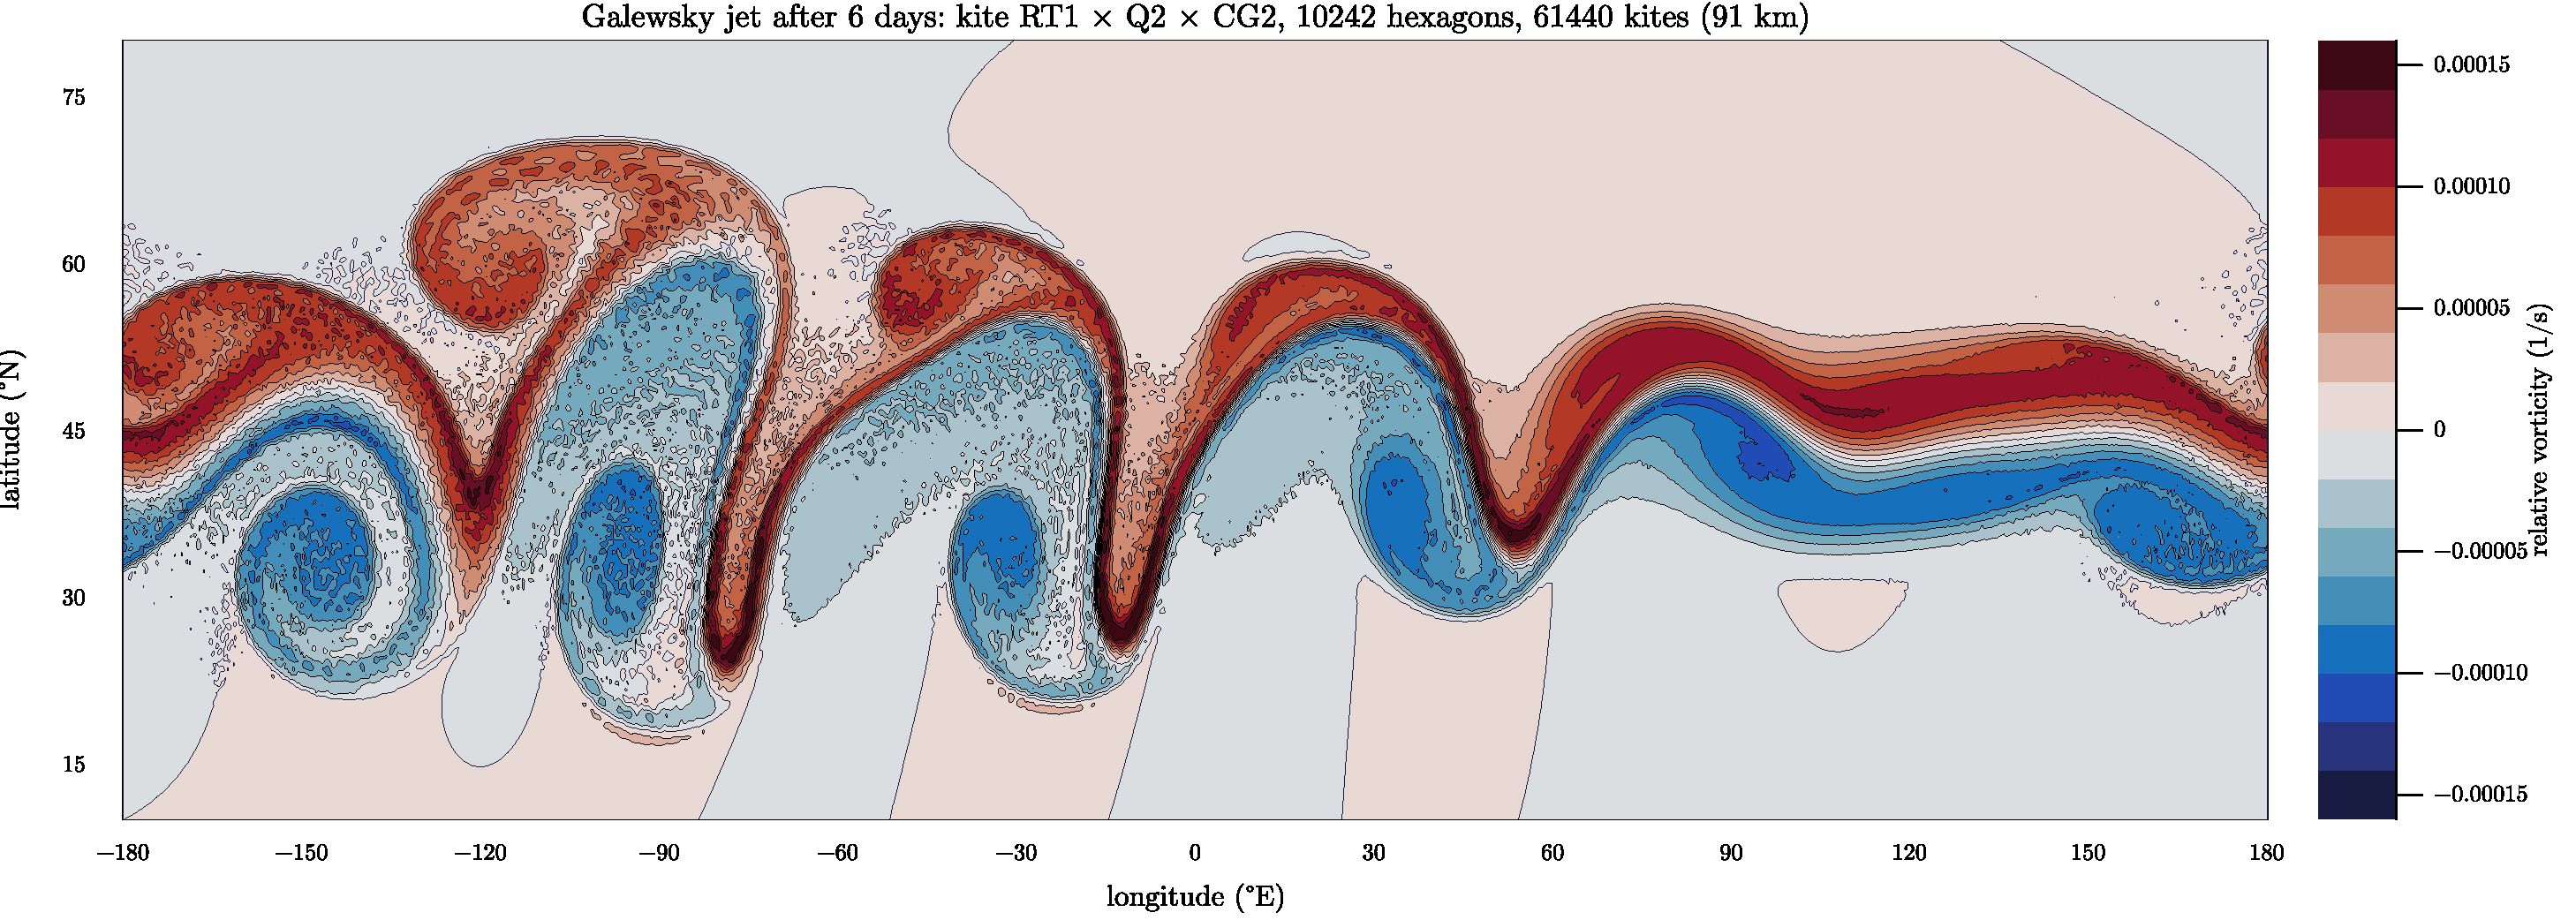
\includegraphics[width=\textwidth]{figures/kite_galewsky.pdf}
\caption{Galewsky jet, relative vorticity after 6 days, $\mathrm{RT}_1\times Q_2\times\mathrm{CG}_2$ on
10\,242 hexagons (61\,440 kites), no dissipation.}
\label{fig:galewsky}
\end{figure}

\paragraph{Bickley jet} A doubly periodic $[0,4\pi)^2$, $u = \mathrm{sech}^2(y-2\pi)$, no rotation, Froude
number 0.2, perturbed in wavenumber~1. On $64\times64$ quadrilaterals (16\,384 kites) the jet forms a
vortex street with two cat's-eye pairs by $t = 40$ (Figure~\ref{fig:bickley}); mass and energy change by
$1.6\cdot10^{-10}$ and $7\cdot10^{-11}$.

\begin{figure}[t]
\centering
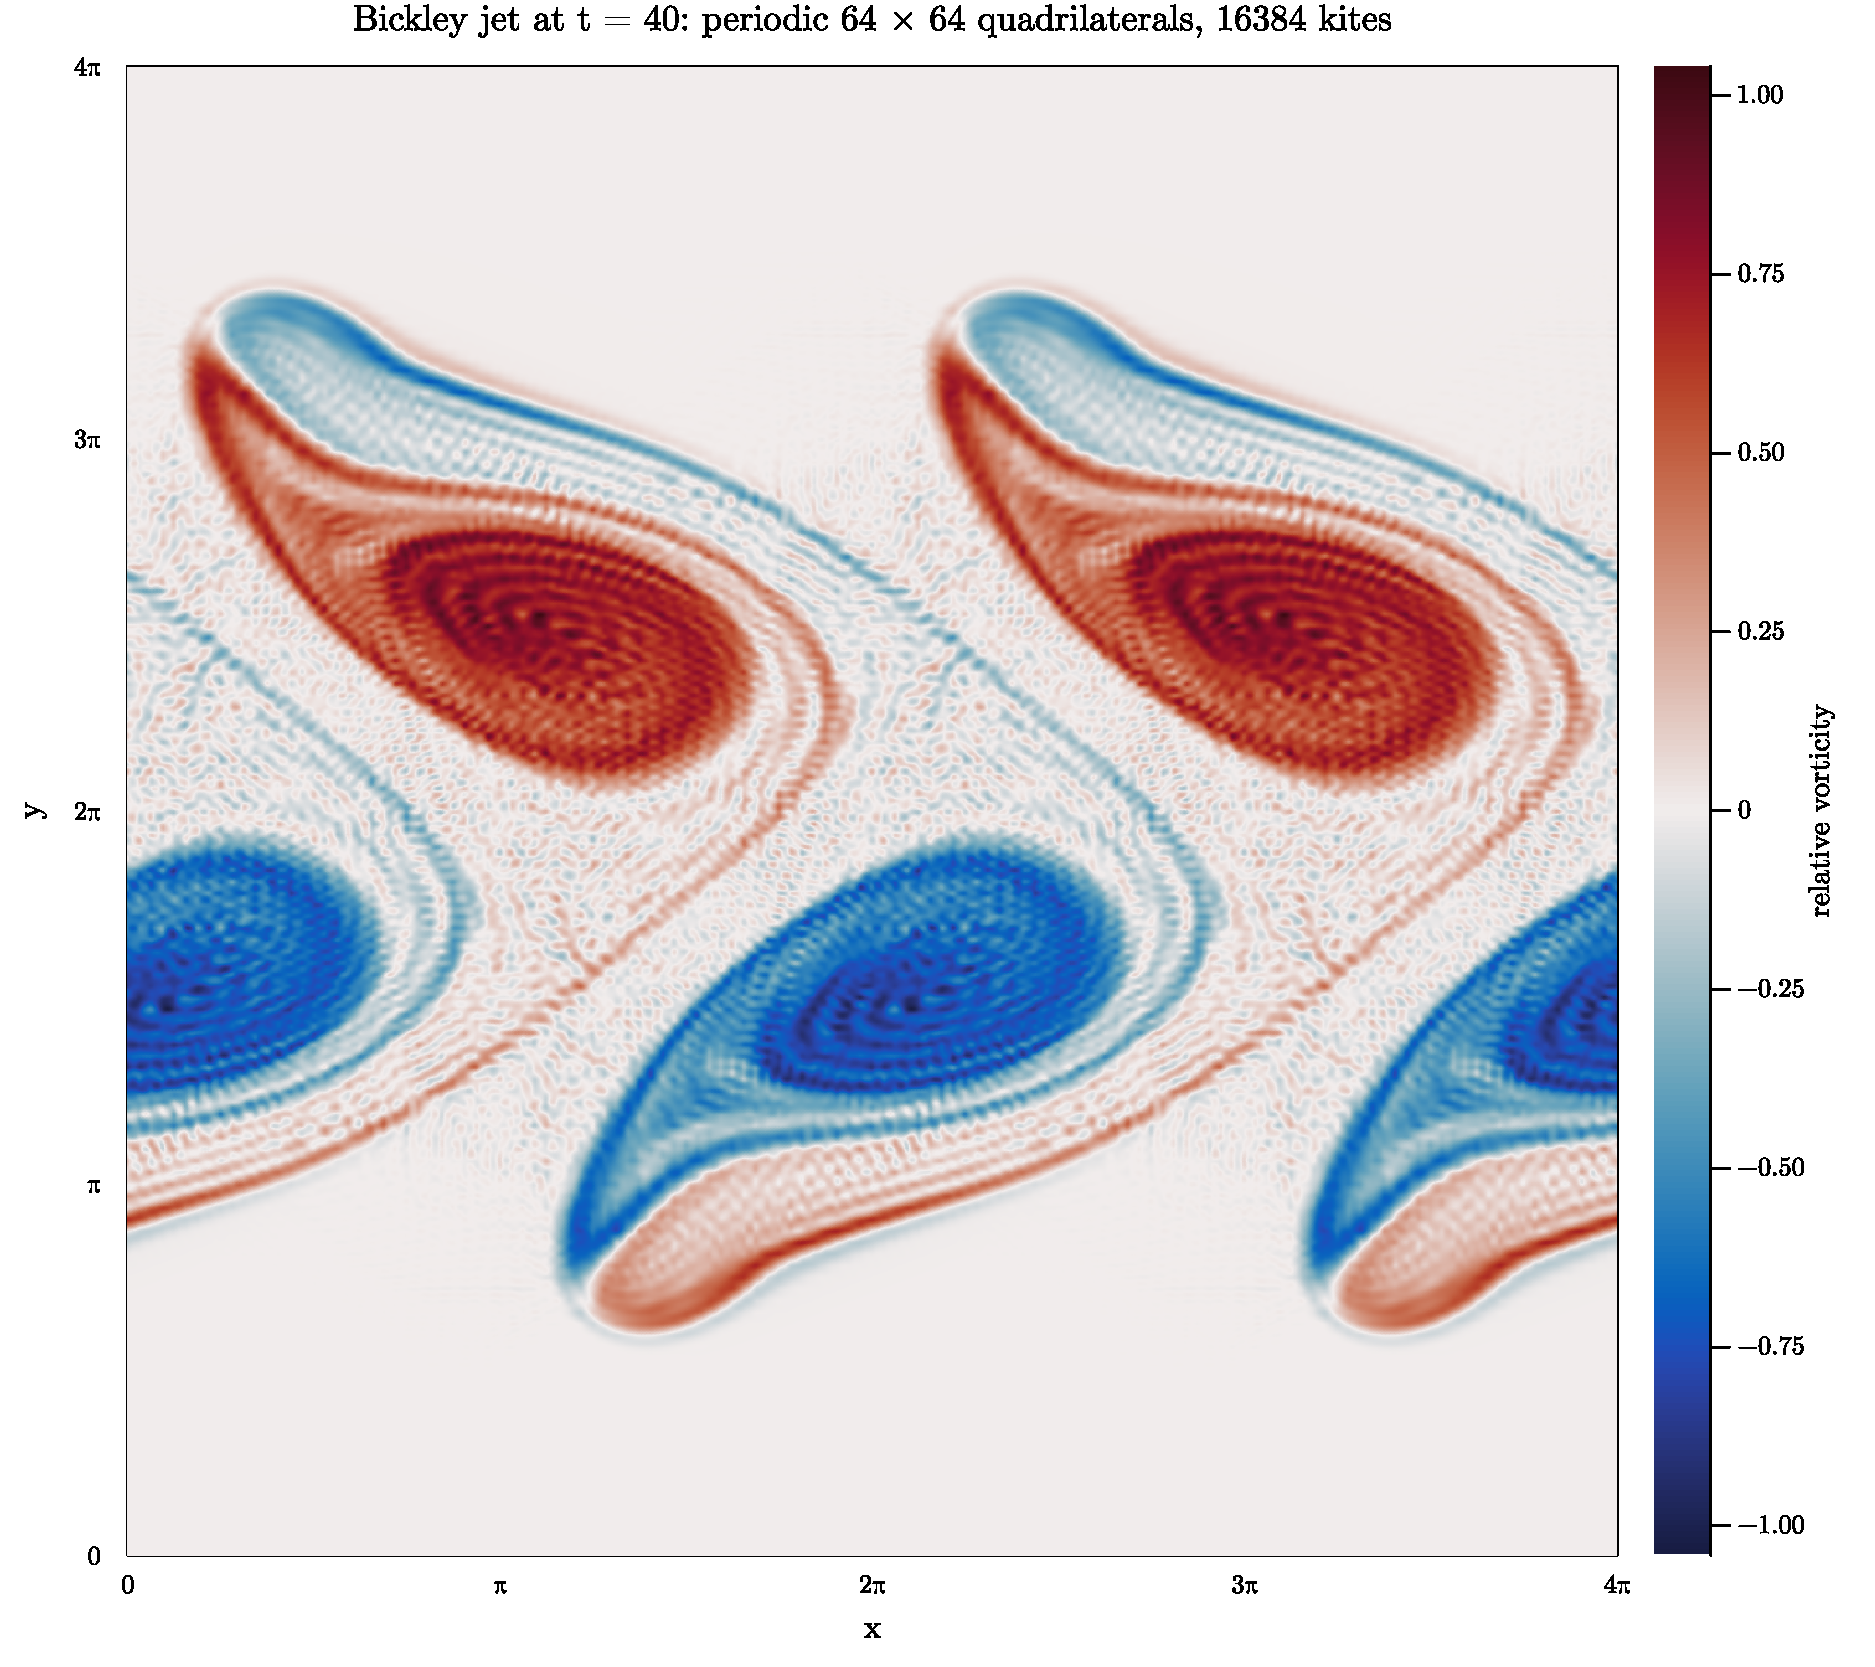
\includegraphics[width=0.75\textwidth]{figures/kite_bickley.pdf}
\caption{Bickley jet, relative vorticity at $t = 40$ on $64\times64$ quadrilaterals (16\,384 kites), no
dissipation.}
\label{fig:bickley}
\end{figure}

%==============================================================================
\section{The compressible Euler equations}\label{sec:3d}

\subsection{Equations}
The dry compressible Euler equations of a shallow atmosphere over flat ground, in height coordinates,
with the horizontal velocity $\bu$, the vertical velocity $w$, the density $\rho$, the potential
temperature $\theta$ and the Exner pressure $\pi = (R\rho\theta/p_0)^{R/c_v}$, are
\begin{align}
  \partial_t \bu &= -(\zeta + f)\,\rhat \times \bu - w\,\partial_z\bu - \nabla K - c_p\theta\nabla\pi, \\
  \partial_t w &= -\bu\cdot\nabla w - w\,\partial_z w - c_p\theta\,\partial_z\pi - g,\\
  \partial_t \rho &= -\nabla\cdot(\rho \bu) - \partial_z(\rho w), \qquad
  \partial_t(\rho\theta) = -\nabla\cdot(\rho\theta \bu) - \partial_z(\rho\theta w),
\end{align}
with $K = \tfrac12|\bu|^2$, between the ground $z = 0$ and a rigid lid $z = z_T$, with $w = 0$ at both.
They are the shallow-atmosphere equations with the traditional approximation: the distance from the centre
is replaced by the radius $a$ in all layers, $f = 2\Omega\sin\varphi$ is the only Coriolis term, and the
metric terms $u^2/r$ of the $w$ equation and $uw/r$ of the $\bu$ equation are dropped. This is the
consistent shallow system that conserves energy and angular momentum \cite{White2005}; all 3D test cases
below are steady states or perturbed steady states of exactly this system. A deep atmosphere, with
$r = a + z$ in the metric and the full Coriolis vector, changes the extruded spaces only through the
weights $r^2$ in the vertical inner products and $1/r$ in the horizontal operators of each layer. They
conserve the total energy
$\int\rho(\tfrac12|\bu|^2 + \tfrac12w^2 + c_v\theta\pi + gz)$, in which $c_v\rho\theta\pi$ is the internal
energy and $\partial(c_v\rho\theta\pi)/\partial(\rho\theta) = c_p\pi$.

\subsection{Extruded spaces}
The vertical grid has the interfaces $0 = z_{1} < z_{2} < \dots < z_{L+1} = z_T$ (index $j$), the layers
$(z_k, z_{k+1})$ of thickness $\Delta z_k$ with centres $\bar z_k$ (index $k$), and the interface thickness
$\Delta z^h_j = \bar z_j - \bar z_{j-1} = (\Delta z_{j-1}+\Delta z_j)/2$. In the vertical, $\mathrm{DG}_0$ is
spanned by the indicator functions $\chi_k$ of the layers and $\mathrm{CG}_1$ by the hat functions $\phi_j$
of the interfaces, with $\phi_1, \phi_{L+1}$ removed for $w = 0$. The 3D spaces are
\begin{center}
\begin{tabular}{lll}
\toprule
field & space & degrees of freedom \\
\midrule
$\rho$, $\rho\theta$ & $W_3 = H_p\otimes\mathrm{DG}_0$ & Radau nodes $\times$ layers \\
$w$ & $H_p\otimes\mathrm{CG}_1$ & Radau nodes $\times$ interior interfaces \\
$\bu$ & $U_k\otimes\mathrm{DG}_0$ & velocity degrees of freedom $\times$ layers \\
\bottomrule
\end{tabular}
\end{center}
Since $\partial_z\mathrm{CG}_1 = \mathrm{DG}_0$, the 3D velocity space
$W_2 = (U_k\otimes\mathrm{DG}_0)\oplus(H_p\otimes\mathrm{CG}_1)$ is mapped by the discrete divergence onto
$W_3$, as in the compatible extruded elements \cite{NataleShiptonCotter2016,Melvin2019}, with the
horizontal part $B$ and the vertical part $\partial_z$. $\theta$ lives with $\rho$ in the layers (Lorenz
staggering). The inner products are tensor products of the lumped rule \eqref{eq:lumped} with the
trapezoidal rule of every layer, the Gauss--Lobatto rule of $\mathrm{CG}_1$. Both have their nodes at
the degrees of freedom, so every Radau node carries one column of $\rho$, $\rho\theta$ and $w$ that is
coupled to the others only by the horizontal terms. This is the vertical counterpart of the mass lumping in
the horizontal, and it is what a HEVI time step needs.

\subsection{Horizontal terms}
Per layer the horizontal terms are those of the shallow-water scheme \eqref{eq:sw} with $\rho$ in place of
$h$:
\begin{equation}\label{eq:vi}
\begin{gathered}
  M_u\dot\bu = -\tfrac1a B^T K - \Bigl(\int \tfrac{\zeta + f}{\rho}\,(\rhat\times\bF)\cdot\bv_j\Bigr)_j
     - c_p\,M_u\,\Pi_U\bigl(\theta\, M_u^{-1}B^T\pi/a\bigr),\\
  \bF = \Pi_U(\rho\bu),\qquad M_h\dot\rho = B\bF/a,\qquad M_h\dot{(\rho\theta)} = B\,\Pi_U(\theta\bF)/a .
\end{gathered}
\end{equation}
With $E = \sum_k\Delta z_k\bigl[\int\rho|\bu|^2/2 + \sum_i M_{h,ii}(c_v\rho\theta\,\pi + \rho g \bar z_k)_i\bigr]$
one has $\partial E/\partial\bu = M_u\bF$, $\partial E/\partial\rho = M_h(K + g\bar z)$ and
$\partial E/\partial(\rho\theta) = M_h c_p\pi$, and the horizontal terms exchange energy without loss, since
the pressure pair cancels through the symmetric $\Theta = (\int\theta\,\bv_i\cdot\bv_j)$. The vertical
coupling $-\boldsymbol\eta w$ with the horizontal vorticity $\boldsymbol\eta = \partial_z\bu - \nabla w$ and
its counterpart $\boldsymbol\eta\cdot\bu$ in the $w$ equation are discretized as exact adjoints.
Section~\ref{sec:2d3d} shows that \eqref{eq:vi} is not sufficient in three dimensions;
Section~\ref{sec:dg} replaces the transport terms.

\subsection{Vertical terms as a Galerkin method}\label{sec:vertical}
Fix a Radau node $i$ and drop the index; the horizontal mass $M_{h,ii}$ multiplies every term of the column
and cancels. All vertical integrals use the trapezoidal rule of each layer.

\paragraph{Mass flux} The vertical mass flux is the lumped $L^2$ projection of $\rho w$ into $\mathrm{CG}_1$,
$F = \Pi_{\mathrm{CG}_1}(\rho w)$, the vertical counterpart of $\bF = \Pi_U(\rho\bu)$. Testing with $\phi_j$,
\[
  \Delta z^h_j F_j = \tfrac12\Delta z_{j-1}\rho_{j-1}w_j + \tfrac12\Delta z_j\rho_jw_j ,
\]
so that
\[
  F_j = \bar\rho_j w_j,\qquad \bar\rho_j = \frac{\Delta z_{j-1}\rho_{j-1} + \Delta z_j\rho_j}{\Delta z_{j-1}+\Delta z_j},
\]
with the thickness-weighted interface mean $\bar\rho_j$. The flux of $\rho\theta$ is
$G = \Pi_{\mathrm{CG}_1}(\theta F)$, $G_j = \bar\theta_jF_j$, with the same mean of $\theta$.

\paragraph{Continuity} Testing $\partial_t\rho + \partial_zF = 0$ with $\chi_k$ is exact, since
$\partial_zF\in\mathrm{DG}_0$:
\[
  \Delta z_k\dot\rho_k = -(F_{k+1} - F_k),\qquad \Delta z_k\dot{(\rho\theta)}_k = -(G_{k+1} - G_k),
\]
with $F_1 = F_{L+1} = 0$. In matrix form $M_3\dot\rho = -D_zF$ with $M_3 = \mathrm{diag}(\Delta z_k)$ and
$(D_zF)_k = F_{k+1} - F_k$.

\paragraph{Vertical momentum} The pressure gradient is the adjoint of the divergence, weighted with $\theta$
as in the horizontal. The discrete vertical gradient of $\pi\in\mathrm{DG}_0$ is
$-M_2^{-1}D_z^T\pi$ with the lumped mass $M_2 = \mathrm{diag}(\Delta z^h_j)$, i.e.\
$(\pi_j - \pi_{j-1})/\Delta z^h_j$, and its product with $\theta$ is projected into $\mathrm{CG}_1$ with the
same rule:
\[
  \Delta z^h_j\dot w_j = -c_p\bar\theta_j(\pi_j - \pi_{j-1}) - g\Delta z^h_j - \Delta z^h_jr_jw_j ,
\]
where $r_j$ is the absorbing layer of Klemp et al.\ \cite{Klemp2008} below the lid. These are the formulas
of a finite-difference Lorenz grid, but every weight is fixed by the Galerkin method: the interface means are
the projections of the trapezoidal rule, $\Delta z^h_j$ is the lumped mass, and the pressure gradient is the
adjoint of the divergence.

\begin{theorem}\label{thm:vertical-energy}
Without damping, the vertical terms exchange energy exactly: with $\partial E/\partial w = M_2F$,
\[
  \sum_j\Delta z^h_jF_j\dot w_j + \sum_k\Delta z_k\bigl(c_p\pi_k\dot{(\rho\theta)}_k + g\bar z_k\dot\rho_k\bigr) = 0 .
\]
\end{theorem}
\begin{proof}
Summation by parts with $F_1 = F_{L+1} = 0$ gives
$\sum_k c_p\pi_k\Delta z_k\dot{(\rho\theta)}_k = -c_p\sum_k\pi_k(G_{k+1}-G_k) = c_p\sum_j\bar\theta_jF_j(\pi_j-\pi_{j-1})$,
which cancels the pressure term of $\sum_j\Delta z^h_jF_j\dot w_j$, and
$\sum_kg\bar z_k\Delta z_k\dot\rho_k = g\sum_jF_j(\bar z_j - \bar z_{j-1}) = g\sum_j\Delta z^h_jF_j$, which cancels
the gravity term.
\end{proof}
The proof needs the same rule in the mass of $w$, in the flux $F$ and in the means $\bar\theta$: the
consistent $\mathrm{CG}_1$ mass of $w$ with the lumped flux, or an upwind $\theta$ in the flux with the mean
$\bar\theta$ in the pressure gradient, break the identity. This is the vertical form of the quadrature
condition of Section~\ref{sec:quadrature-mismatch}.

\paragraph{Upwinding} The central flux $\bar\theta_jF_j$ is the DG$_0$ flux with the mean trace. An upwind
option adds the penalty $P_j = \alpha|F_j|(\theta_{j-1} - \theta_j)/2$, which for $\alpha = 1$ and
equidistant layers turns $\bar\theta_jF_j + P_j$ into the upwind flux. The penalty does not change $\rho$
and damps the variance of $\theta$, at the cost of the exact energy exchange.
% TODO: choose the default (central / upwind) from the comparison runs; state it here.

\paragraph{Tracers} A tracer $\rho q$ is transported with the same flux, $Q_j = \bar q_jF_j$ (plus the
penalty), so that $q = 1$ reproduces the continuity equation.

\subsection{Time discretization}\label{sec:time}
The time step is the Wicker--Skamarock RK3 scheme \cite{WickerSkamarock2002} with the stages
$\tau = \Delta t/3, \Delta t/2, \Delta t$, each a HEVI step from the state $y^n$ with the tendencies of the
stage state $y^s$:
\begin{enumerate}
\item explicit horizontal momentum, $\bu = \bu^n + \tau\,T_u(y^s)$;
\item forward--backward horizontal transport with the new velocity and $\rho^s$, $\theta^s$: the explicit
  parts $\rho^\ast$, $(\rho\theta)^\ast$;
\item one implicit Galerkin step of the vertical terms of Section~\ref{sec:vertical} in every column.
\end{enumerate}
The implicit step freezes the interface means $\bar\rho_j$, $\bar\theta_j$ and the penalty $P_j$ at the stage
state, off-centres the vertical velocity with $\beta$, $w^\beta_j = \beta w_j + (1-\beta)w^n_j$, and
linearizes the Exner pressure around $y^n$, $\pi = \pi^n + \gamma^n(\rho\theta - (\rho\theta)^n)$ with
$\gamma^n = (R/c_v)\pi^n/(\rho\theta)^n$:
\begin{gather*}
  \rho_k = \rho^\ast_k - \frac{\tau}{\Delta z_k}(F_{k+1} - F_k),\qquad
  (\rho\theta)_k = (\rho\theta)^\ast_k - \frac{\tau}{\Delta z_k}(G_{k+1} - G_k),\\
  F_j = \bar\rho_jw^\beta_j,\qquad G_j = \bar\theta_jF_j + P_j,\\
  w_j = w^n_j + \tau\bigl(T_{w,j}(y^s) - g - r_jw_j\bigr)\\
  - \frac{\tau c_p\bar\theta_j}{\Delta z^h_j}\bigl[\beta(\pi_j - \pi_{j-1}) + (1-\beta)(\pi^n_j - \pi^n_{j-1})\bigr].
\end{gather*}
Inserting $(\rho\theta)_k$ into the linearized $\pi$ leaves one tridiagonal system in $w$ per column. The
flux $F_j$ of the solved $w$ is the one of the continuity, $\rho\theta$ and tracer equations, so mass is
conserved to round-off and $q = 1$ stays exactly $1$. The default is $\beta = 0.65$.

\paragraph{Discrete hydrostatic balance} The initial columns solve the discrete balance of the column step,
$c_p\bar\theta_j(\pi_j - \pi_{j-1}) = -g\Delta z^h_j$, upwards from the lowest layer by a fixed-point
iteration for $\pi_j$ with the given temperature, so that an atmosphere at rest stays at rest to
round-off.

\subsection{Orography: options for the vertical discretization}\label{sec:orography}
% Draft of the design options; not implemented in the kite model yet.
Over orography the levels follow the terrain, $z = \zeta + h(\mathbf{x})\,b(\zeta)$ over reference levels
$0 = \zeta_1 < \dots < \zeta_{L+1} = z_T$, with $b(0) = 1$ and $b = 0$ above a height $z_F \le z_T$. The basic
coordinate $b = 1 - \zeta/z_T$ \cite{GalChen1975} and the smooth decay
$b = \sinh((z_F/s)^n - (\zeta/s)^n)/\sinh((z_F/s)^n)$ \cite{Schaer2002} are the usual choices. The layer
thickness $\Delta z_k(\mathbf{x})$ now depends on the position, and the extruded element of a kite and a layer is a
prism with a sloping top and bottom. The column structure of Section~\ref{sec:vertical} survives unchanged:
every Radau node $i$ carries its own column with the thicknesses $\Delta z_k(\mathbf{x}_i)$, its mass, fluxes and
pressure gradient are those of a flat column with these thicknesses, and Theorem~\ref{thm:vertical-energy}
holds column by column. What changes is the horizontal part and the coupling of the two.

\paragraph{Mass flux and continuity} With the reference coordinate $\zeta$ the continuity equation of layer $k$
is $\partial_t(\Delta z_k\rho_k) + \nabla_\zeta\cdot(\Delta z_k\rho_k\bu_k) + (\Omega_{k+1} - \Omega_k) = 0$,
with the mass flux $\Omega_j$ through the sloping interface, $\Omega_j = F_j - \overline{\rho\,\bu\cdot\nabla z}_j$.
At the Radau nodes $\Delta z_k(\mathbf{x}_i)$ is a diagonal factor of the height mass, so $\rho$, $\rho\theta$ and $w$
keep diagonal masses $M_{h,ii}\Delta z_k(\mathbf{x}_i)$ and $M_{h,ii}\Delta z^h_j(\mathbf{x}_i)$. The correction
$\bu\cdot\nabla z$ at the nodes needs the pointwise velocity and the gradient of the levels, both available in
the height space; the lower boundary condition becomes $\Omega_1 = 0$, that is $w = \bu\cdot\nabla h$ at the
ground.

\paragraph{Pressure gradient} On the sloping levels $\nabla_z\pi = \nabla_\zeta\pi - \nabla z\,\partial_z\pi$. As the
adjoint of the divergence of the transformed equations the metric term follows from the Galerkin method; the
truncation error over steep slopes is reduced by writing it for the deviation $\pi' = \pi - \pi_\mathrm{ref}(z)$
from a reference profile, whose gradient on height surfaces vanishes.

\paragraph{The velocity mass} The energy is now
$E = \sum_k\int\Delta z_k(\mathbf{x})\bigl[\rho|\bu|^2/2 + c_v\rho\theta\pi + \rho g\bar z_k\bigr]$, so the exact energy
exchange of the horizontal terms needs $\partial E/\partial\bu = M_u^{(k)}\bF$ with the thickness-weighted mass
$M_u^{(k)} = \bigl(\int\Delta z_k\,\bv_i\cdot\bv_j\bigr)$ of every layer, and the projection $\Pi_U$ of the fluxes
with the same weighted rule (Section~\ref{sec:quadrature-mismatch}). There are three options.
\begin{enumerate}
\item \emph{Weighted mass per layer.} $M_u^{(k)}$ in every layer, with the rule of the projections. Energy and
  the Casimir property of Section~\ref{sec:quadrature-mismatch} are kept, but the dual-cell blocks are
  factorized $L$ times, which multiplies the storage of the factors and their set-up by the number of layers.
\item \emph{Separable thickness.} If $\Delta z_k(\mathbf{x}) = \Delta\zeta_k\,J(\mathbf{x})$, as for the basic coordinate with
  $J = 1 - h/z_T$, then $M_u^{(k)} = \Delta\zeta_k M_u^J$ with the single weighted mass
  $M_u^J = (\int J\,\bv_i\cdot\bv_j)$. One factorization serves all layers and option 1 costs no more than flat
  ground. A smooth decay of the terrain with height is not separable; a coordinate that is separable in a
  few height zones keeps the number of factorizations at the number of zones.
\item \emph{Flat velocity mass.} $M_u$ of the reference levels, the thickness only in the diagonal height mass and
  in the fluxes. This is the choice of finite-volume C-grid models; it is cheap but gives up the exact energy
  exchange and $\Pi_U(c\bv) = c\bv$ for the weighted fluxes, and with it the protection of the stratified rest
  state against the sub-cell mode of Section~\ref{sec:quadrature-mismatch}.
\end{enumerate}

\paragraph{Static condensation of the kite blocks} The cost of option 1 is dominated by the factorization of
the dual-cell blocks. A dual-cell block couples its kites only through the $s$ normal degrees of freedom of
their common primal faces (Section~\ref{sec:quadrature-mismatch}). On every kite the remaining
$m - 2s$ unknowns, the interior ones and those of the two dual faces, can be eliminated by a local Schur
complement. What remains per dual cell is a cyclic block-tridiagonal system of $n_w s$ face unknowns, six for
$U_1$ on a hexagonal mesh in place of thirty. The interior solves are independent of the dual cell and of $n_w$:
they are small dense systems of one size for all kites of all meshes, ideal for batched solves on GPUs,
and the same matrix for congruent kites. With a weight that varies from layer to layer only the small
interior inverses and the face system have to be recomputed, which can be done on the fly in every layer
instead of storing $L$ factors.

%==============================================================================
\section{From two to three dimensions}\label{sec:2d3d}

The 3D model with \eqref{eq:vi} conserves energy and keeps the rest state, but is unstable in a flow,
although every shallow-water test passes. The 3D model is a tensor product, but four properties that are
irrelevant or hidden in shallow water become essential:
\begin{enumerate}
\item the consistency of the quadrature of the velocity mass with the projections
  (Section~\ref{sec:quadrature-mismatch});
\item the skew-symmetry of the projected transport of scalars without a gravity-wave feedback
  (Section~\ref{sec:projected});
\item the stability of the momentum transport in flow faster than the gravity waves
  (Section~\ref{sec:supercritical});
\item the different weighting of the sub-cell height modes by the horizontal and the vertical pressure
  gradient (Section~\ref{sec:submodes}).
\end{enumerate}
Two further points are inherited from the vertical discretization: the Lorenz staggering of $\theta$ has a
computational mode in the potential temperature \cite{ArakawaMoorthi1988,ThuburnWoollings2005}, and the
vertical order is one below the horizontal one. The tool of the analysis is the spectrum of the linearized
horizontal tendency of one layer; max $\mathrm{Re}\,\lambda>0$ is a growing mode of the semi-discrete
equations, independent of the time step.

\subsection{Quadrature of the velocity mass}\label{sec:quadrature-mismatch}
The velocity mass was first assembled with an exact rule (degree 6), the projections $\Pi_U(h\bv)$ with the
$3\times3$ rule of the nonlinear terms. On non-affine kites the metric $J^TJ/\det J$ is rational, the two
differ, and $\Pi_U(c\,\bv)\ne c\,\bv$ for a constant $c$ ($1.4\cdot10^{-2}$ on hexagon kites). Then the
$\rho\theta$ flux $\Pi_U(\bar\theta\bF)$ is not $\bar\theta$ times the mass flux: the horizontal fluxes create
sub-cell entropy at rest. The energy is still conserved, but the Casimir $\int\rho f(\theta)$ that makes the
stratified rest state stable is not, and a sub-cell mode lives on the released potential energy. On the
affine kites of the cubed sphere both rules are exact and the mode is absent. Assembling $M_u$ with the rule
of the projections restores $\Pi_U(c\,\bv) = c\,\bv$ to round-off and removes the mode. In shallow water there
is no second scalar, and the defect is invisible.

With this rule the blocks of $M_u$ are no longer the $2\times2$ node blocks of the lumped mass of
\cite{Wess2024} but the full dual-cell blocks of Table~\ref{tab:dofs}, also for the $Q_p^2$ space. They are
sparse. A basis function couples only with the functions of its own kite, and two kites of a dual cell share
only the $s$ normal degrees of freedom of their common primal face ($s = k+1$ for $\mathrm{RT}_k$ and
$\mathrm{BDM}_k$, $s = p+1$ for $Q_p^2$). The graph of a block with $n_w$ kites is therefore a ring of $n_w$
cliques of $m = n/n_w + s$ unknowns that overlap in the face unknowns, with
\[
  \mathrm{nnz}(A) = n_w\Bigl(\tfrac{m(m+1)}{2} - \tfrac{s(s+1)}{2}\Bigr)
\]
entries in the lower triangle, about $3/(2n_w)$ of the dense triangle. Numbered kite by kite, the Cholesky
factor $L$ gets fill only where the ring closes: $s^2$ entries for every kite beyond the third, so
$\mathrm{nnz}(L) = \mathrm{nnz}(A) + s^2(n_w - 3)$. A dual cell of three kites (hexagonal meshes) has no fill at
all, because every two faces of it belong to a common kite. A minimum-degree ordering (CHOLMOD) gives the same
counts. Table~\ref{tab:blocks} lists the blocks for the dual cells of the three meshes: the triangles and
pentagons of the dual cells of icosahedral triangle meshes ($n_w = 6, 5$), the quadrilaterals of the cubed
sphere ($n_w = 4$) and the triangles of hexagonal meshes ($n_w = 3$).

The sparse factor is computed once, because $M_u$ does not change in time. A solve with it, one forward and
one backward substitution per block and layer, reads $2\,\mathrm{nnz}(L)$ values instead of the $n^2$ of the
dense inverse, 3 to 4.5 times fewer for $n_w \ge 5$ and about 2 times for $n_w = 3$. The factorization
itself costs $\sum_j c_j^2$ multiply-adds ($c_j$ the entries of column $j$ of $L$) instead of $n^3/3$, 3 to 22
times fewer, the more the larger the block.
That matters where a block has to be factorized in every stage, as the density-weighted mass of
Section~\ref{sec:dg}. All blocks of one kind of dual cell have the same pattern up to the numbering of
their unknowns: with the kites and their unknowns numbered in the same order in every dual cell, the blocks
can be sorted by $n_w$ and the symbolic factorization done once per kind, as in batched solvers for many
small systems of one pattern \cite{Abdelfattah2017}. Only the values of $L$ are then stored per block, layers
first, so that the threads of the layers of one block read the same pattern and adjacent values.

\begin{table}[t]
\centering
\caption{Dual-cell blocks of the velocity mass with the rule of the projections, for $n_w$ kites per dual
cell: size $n$, nonzeros of the lower triangle of the block $A$ and of its Cholesky factor $L$ (kite-by-kite
numbering; the fill is $s^2(n_w-3)$), of the dense lower triangle, multiply-adds of the factorization
($\sum_j c_j^2$ sparse, $n^3/3$ dense) and values read by a solve ($2\,\mathrm{nnz}(L)$ with the sparse factor,
$n^2$ with the dense inverse). $\mathrm{BDM}_1$ and $Q_1^2$ have the same counts.}
\label{tab:blocks}
\footnotesize\setlength{\tabcolsep}{4pt}\begin{tabular}{lrrrrrrr}
\toprule
space & $n_w$ & $n$ & $\mathrm{nnz}(A)$ & $\mathrm{nnz}(L)$ & dense & factorization & solve \\
\midrule
$\mathrm{BDM}_1$, $Q_1^2$ ($s = 2$) & 3 & 18 & 99 & 99 & 171 & 613 / 1944 & 198 / 324 \\
 & 4 & 24 & 132 & 136 & 300 & 848 / 4608 & 272 / 576 \\
 & 5 & 30 & 165 & 173 & 465 & 1083 / 9000 & 346 / 900 \\
 & 6 & 36 & 198 & 210 & 666 & 1318 / 15552 & 420 / 1296 \\
\midrule
$U_1 = \mathrm{RT}_1$ ($s = 2$) & 3 & 30 & 225 & 225 & 465 & 1951 / 9000 & 450 / 900 \\
 & 4 & 40 & 300 & 304 & 820 & 2632 / 21333 & 608 / 1600 \\
 & 5 & 50 & 375 & 383 & 1275 & 3313 / 41667 & 766 / 2500 \\
 & 6 & 60 & 450 & 462 & 1830 & 3994 / 72000 & 924 / 3600 \\
\midrule
$Q_2^2$ ($s = 3$) & 3 & 45 & 495 & 495 & 1035 & 6339 / 30375 & 990 / 2025 \\
 & 4 & 60 & 660 & 669 & 1830 & 8551 / 72000 & 1338 / 3600 \\
 & 5 & 75 & 825 & 843 & 2850 & 10763 / 140625 & 1686 / 5625 \\
 & 6 & 90 & 990 & 1017 & 4095 & 12975 / 243000 & 2034 / 8100 \\
\midrule
$U_2 = \mathrm{RT}_2$ ($s = 3$) & 3 & 63 & 882 & 882 & 2016 & 14712 / 83349 & 1764 / 3969 \\
 & 4 & 84 & 1176 & 1185 & 3570 & 19715 / 197568 & 2370 / 7056 \\
 & 5 & 105 & 1470 & 1488 & 5565 & 24718 / 385875 & 2976 / 11025 \\
 & 6 & 126 & 1764 & 1791 & 8001 & 29721 / 666792 & 3582 / 15876 \\
\bottomrule
\end{tabular}
\end{table}

\subsection{Projected transport of scalars}\label{sec:projected}
A passive tracer $\rho q$ transported like $\rho\theta$, $M_h\dot{(\rho q)} = B\,\Pi_U(q\bF)/a$, grows exactly
like $\theta'$ in a one-layer flow, although its equation is linear and has no feedback: the transport itself
is unstable. The spectrum of the transport of a height field with a prescribed velocity (Williamson case~2,
$\mathrm{RT}_1\times Q_2$), in units of $u_0/\Delta x$:
\begin{center}
\begin{tabular}{lccc}
\toprule
max $\mathrm{Re}\,\lambda$ & hexagons & cubed sphere & triangles \\
\midrule
projected flux $B\,\Pi_U(\rho\bu)$ & 0.700 & 0.278 & 1.473 \\
pointwise flux, interior trace & 4.757 & 1.245 & 2.428 \\
DG, central trace & 0.001 & 0.000 & 0.002 \\
DG, upwind trace & 0.000 & 0.000 & 0.000 \\
\bottomrule
\end{tabular}
\end{center}
The projected flux tests $\rho\bu$ with the discrete gradient $M_u^{-1}B^T\eta$ of the test function, which
carries the jumps of $\eta$ across primal edges spread over the dual-cell mass blocks, so
$\langle\dot\rho,\eta\rangle + \langle\dot\eta,\rho\rangle\ne\int\bu\cdot\nabla(\rho\eta) = 0$: a consistency
defect at the grid scale, independent of the quadrature (degree 10 changes nothing) and largest on the
irregular kites of triangles. In shallow water and in the 3D model the gravity-wave coupling to the momentum
keeps $\rho$ bounded; a transported quantity without that feedback ($q$, $\theta'$) sees the bare operator.

\subsection{Supercritical flow}\label{sec:supercritical}
With the DG transport of $\theta$ (Section~\ref{sec:dg}) the steady thermal wind still grows in 3D, on all
three meshes and faster on triangles. Ablations show that the growth needs neither shear nor vertical
advection nor rotation, but more than one layer: one layer in solid-body rotation stays at rest, five layers
grow. The internal gravity waves of vertical mode $m$ in an atmosphere of depth $H$ and buoyancy frequency
$N_b$ travel at about $c_m = N_bH/(m\pi)\approx 105/m$\,m/s for $H = 30$\,km, so the higher modes are slower
than the jet. This is reproduced by one layer with a uniform flow $(1, 0.3)$ on the periodic unit square and
the shallow-water equation of state with wave speed $c$: it is stable for $c > |\bu|$ and grows for
$c < |\bu|$, at a rate roughly proportional to $c$. At $c = 0.5$:
\begin{center}\small
\begin{tabular}{lccc}
\toprule
max $\mathrm{Re}\,\lambda\,\Delta x/|\bu|$ & full & momentum ($\rho$ frozen) & continuity ($\bu$ frozen) \\
\midrule
quadrilaterals & 3.49 & 0.77 & 0.77 \\
triangles & 6.08 & 5.48 & 5.49 \\
\bottomrule
\end{tabular}
\end{center}
Both transports of \eqref{eq:vi} are unstable on their own, the vector-invariant momentum transport (PV flux
and $\nabla K$) and the projected continuity $B\,\Pi_U(\rho\bu)$. In subcritical flow the fast gravity-wave
coupling and the conserved energy keep the coupled system neutral; this is why all shallow-water tests (Froude
number below one) and the one-layer 3D tests pass. In supercritical flow the perturbations can draw energy
from the mean flow. In the energy norm $E = \mathrm{diag}(H M_u, g M_h)$ the symmetric part of $EJ$ is
35\,\% of its skew part, almost all of it in the momentum block; the continuity block contributes 0.3\,\%.
Both blocks must be skew-symmetric on their own.

\subsection{Sub-cell height modes}\label{sec:submodes}
For $p = k+1$ the horizontal pressure gradient $B^T\pi$ does not see the component of $\pi$ along the cell
modes $\psi_P$ of Theorem~\ref{thm:kernel}, while the vertical gradient $(\pi_j - \pi_{j-1})/\Delta z^h_j$ acts
on the nodal values and sees every pattern. In shallow water the modes are invariants and stay at the level
of the initial projection. In three dimensions the vertical terms act node by node and change the
coefficients $\psi_P^TM_h\rho$ and $\psi_P^TM_h(\rho\theta)$ of every layer, and a sub-cell pattern of $\pi$
that is created by the vertical terms is not removed by any horizontal pressure force. The DG transport of
Section~\ref{sec:dg} couples the modes to the flow, since its test functions are differentiated inside the
kites with the pointwise velocity.
% TODO: quantify (energy of the psi_P component in the 3D runs); spectra of the 3D linearized operator on few layers.

%==============================================================================
\section{Discontinuous Galerkin transport}\label{sec:dg}

\paragraph{Scalars} $\rho$, $\rho\theta$ and the tracers are transported by
\begin{equation}\label{eq:dg-theta}
  \langle \dot{(\rho q)}, \eta\rangle = \frac1a\Bigl(\sum_K \int_K q\,\bF\cdot\nabla\eta
     - \sum_{F\in\Fc_p} \int_F \hat q\,(\bF\cdot\bn_K)\,\jump{\eta}\Bigr),
\end{equation}
over the primal faces $\Fc_p$ with the central or upwind trace $\hat q$. For $q = 1$ it is $B\bF$, so
$\rho q = \rho$ is kept; it is skew in $q$ (central) or dissipative (upwind). The pressure gradient uses its
adjoint, so the energy exchange stays exact, and the horizontal advection of $w$ is DG in advective form for
the same reason. In the one-layer thermal shallow-water test (Williamson case~2, random
$\theta' = 10^{-8}$) $\theta'$ now stays at $10^{-8}$ on all three meshes, instead of overflowing within a
day on hexagons and triangles.

\paragraph{Momentum and density} With the DG momentum transport, $\rho$, $\rho\theta$ and the tracers are
transported by \eqref{eq:dg-theta} with the pointwise velocity $\bF = \bu$ and $\hat q$ the density trace,
and the momentum equation is solved in advective form with the density-weighted velocity mass:
\begin{multline}\label{eq:dg-u}
  \int \rho\,\dot\bu\cdot\bv = -\frac1a N(\bu;\bv) - \int\rho f\,(\rhat\times\bu)\cdot\bv\\
   - \frac{c_p}{a}\Bigl(\sum_K\int_K\rho\theta\,\bv\cdot\nabla\pi - \sum_{F\in\Fc_p}\int_F\widehat{\rho\theta}\,(\bv\cdot\bn_K)\jump{\pi}\Bigr)\\
   - \sum_{j = k,k+1}\frac{1}{2\Delta z_k}\int \rho\,w_j\,\jump{\bu}_j\cdot\bv ,
\end{multline}
\begin{multline*}
  N(\bu;\bv) = \sum_K\int_K \rho\,\bv\cdot(\bu\cdot\nabla)\bu
  - \sum_{F\in\Fc}\int_F \hat\rho\,\avg{\bu\cdot\bn}\,\jump{\bu}\cdot\avg{\bv}\\
  + \alpha\sum_{F\in\Fc}\int_F \hat\rho\,\frac{|\bu\cdot\bn|}{2}\,\jump{\bu}\cdot\jump{\bv},
\end{multline*}
over all four faces $\Fc$ of every kite (across primal faces only the tangential component jumps, across
dual faces the whole velocity), $\hat\rho$ the mean of the two traces and $\alpha = 1$ for upwinding. The last
term of \eqref{eq:dg-u} is the vertical advection of the $\mathrm{DG}_0$ velocity with the central flux: the
jump $\jump{\bu}_j = \bu_j - \bu_{j-1}$ between the layers $j-1$ and $j$ is shared by the two layers. The pressure term is the
adjoint of the DG $\rho\theta$ transport, so the exchange with the internal energy stays exact. The volume
term is metric free except for the derivative of the Piola factor,
$(\bu\cdot\nabla)\bu\,dA = \sum_k\hat u_k\,\partial_{\xi_k}(P\hat\bu)\,d\xi$ with $P = J/\det J$,
$\partial_{\xi_k}(P\hat\bu) = (\partial_{\xi_k}P)\hat\bu + P\partial_{\xi_k}\hat\bu$, and $\partial_{\xi_k}P$ from
a Richardson extrapolation of central differences of the cell map. The density-weighted mass
$\int\rho\,\bv_a\cdot\bv_b$ is assembled with the rule of the nonlinear terms and factorized per dual cell
(Cholesky), so it stays local.

For uniform $\rho$ and divergence-free $\bu$ the central part of $N$ is skew-symmetric, and the upwind
penalty only removes energy. Since the kinetic energy of the advective form is not exactly the $K$ of the pressure term (the projection
of $K$ into $H_2$), the scheme does not conserve energy exactly; the upwind term supplies the dissipation.

Figure~\ref{fig:spectra} shows the spectra of the one-layer test at $c = 0.5$. The vector-invariant form has
growing modes up to $3.49\,|\bu|/\Delta x$ on quadrilaterals and $6.08\,|\bu|/\Delta x$ on triangles. The DG
form with the central trace is neutral on quadrilaterals and nearly so on triangles (0.014, from the
quadrature on non-affine kites); with the upwind trace max $\mathrm{Re}\,\lambda = 0$ on both. The DG
advection has the explicit limit of DG with RK3, about 0.1 in the advective Courant number per kite; the 3D
runs below are at about 0.02. It costs about 20\,\% more per step than \eqref{eq:vi}.

\begin{figure}[t]
\centering
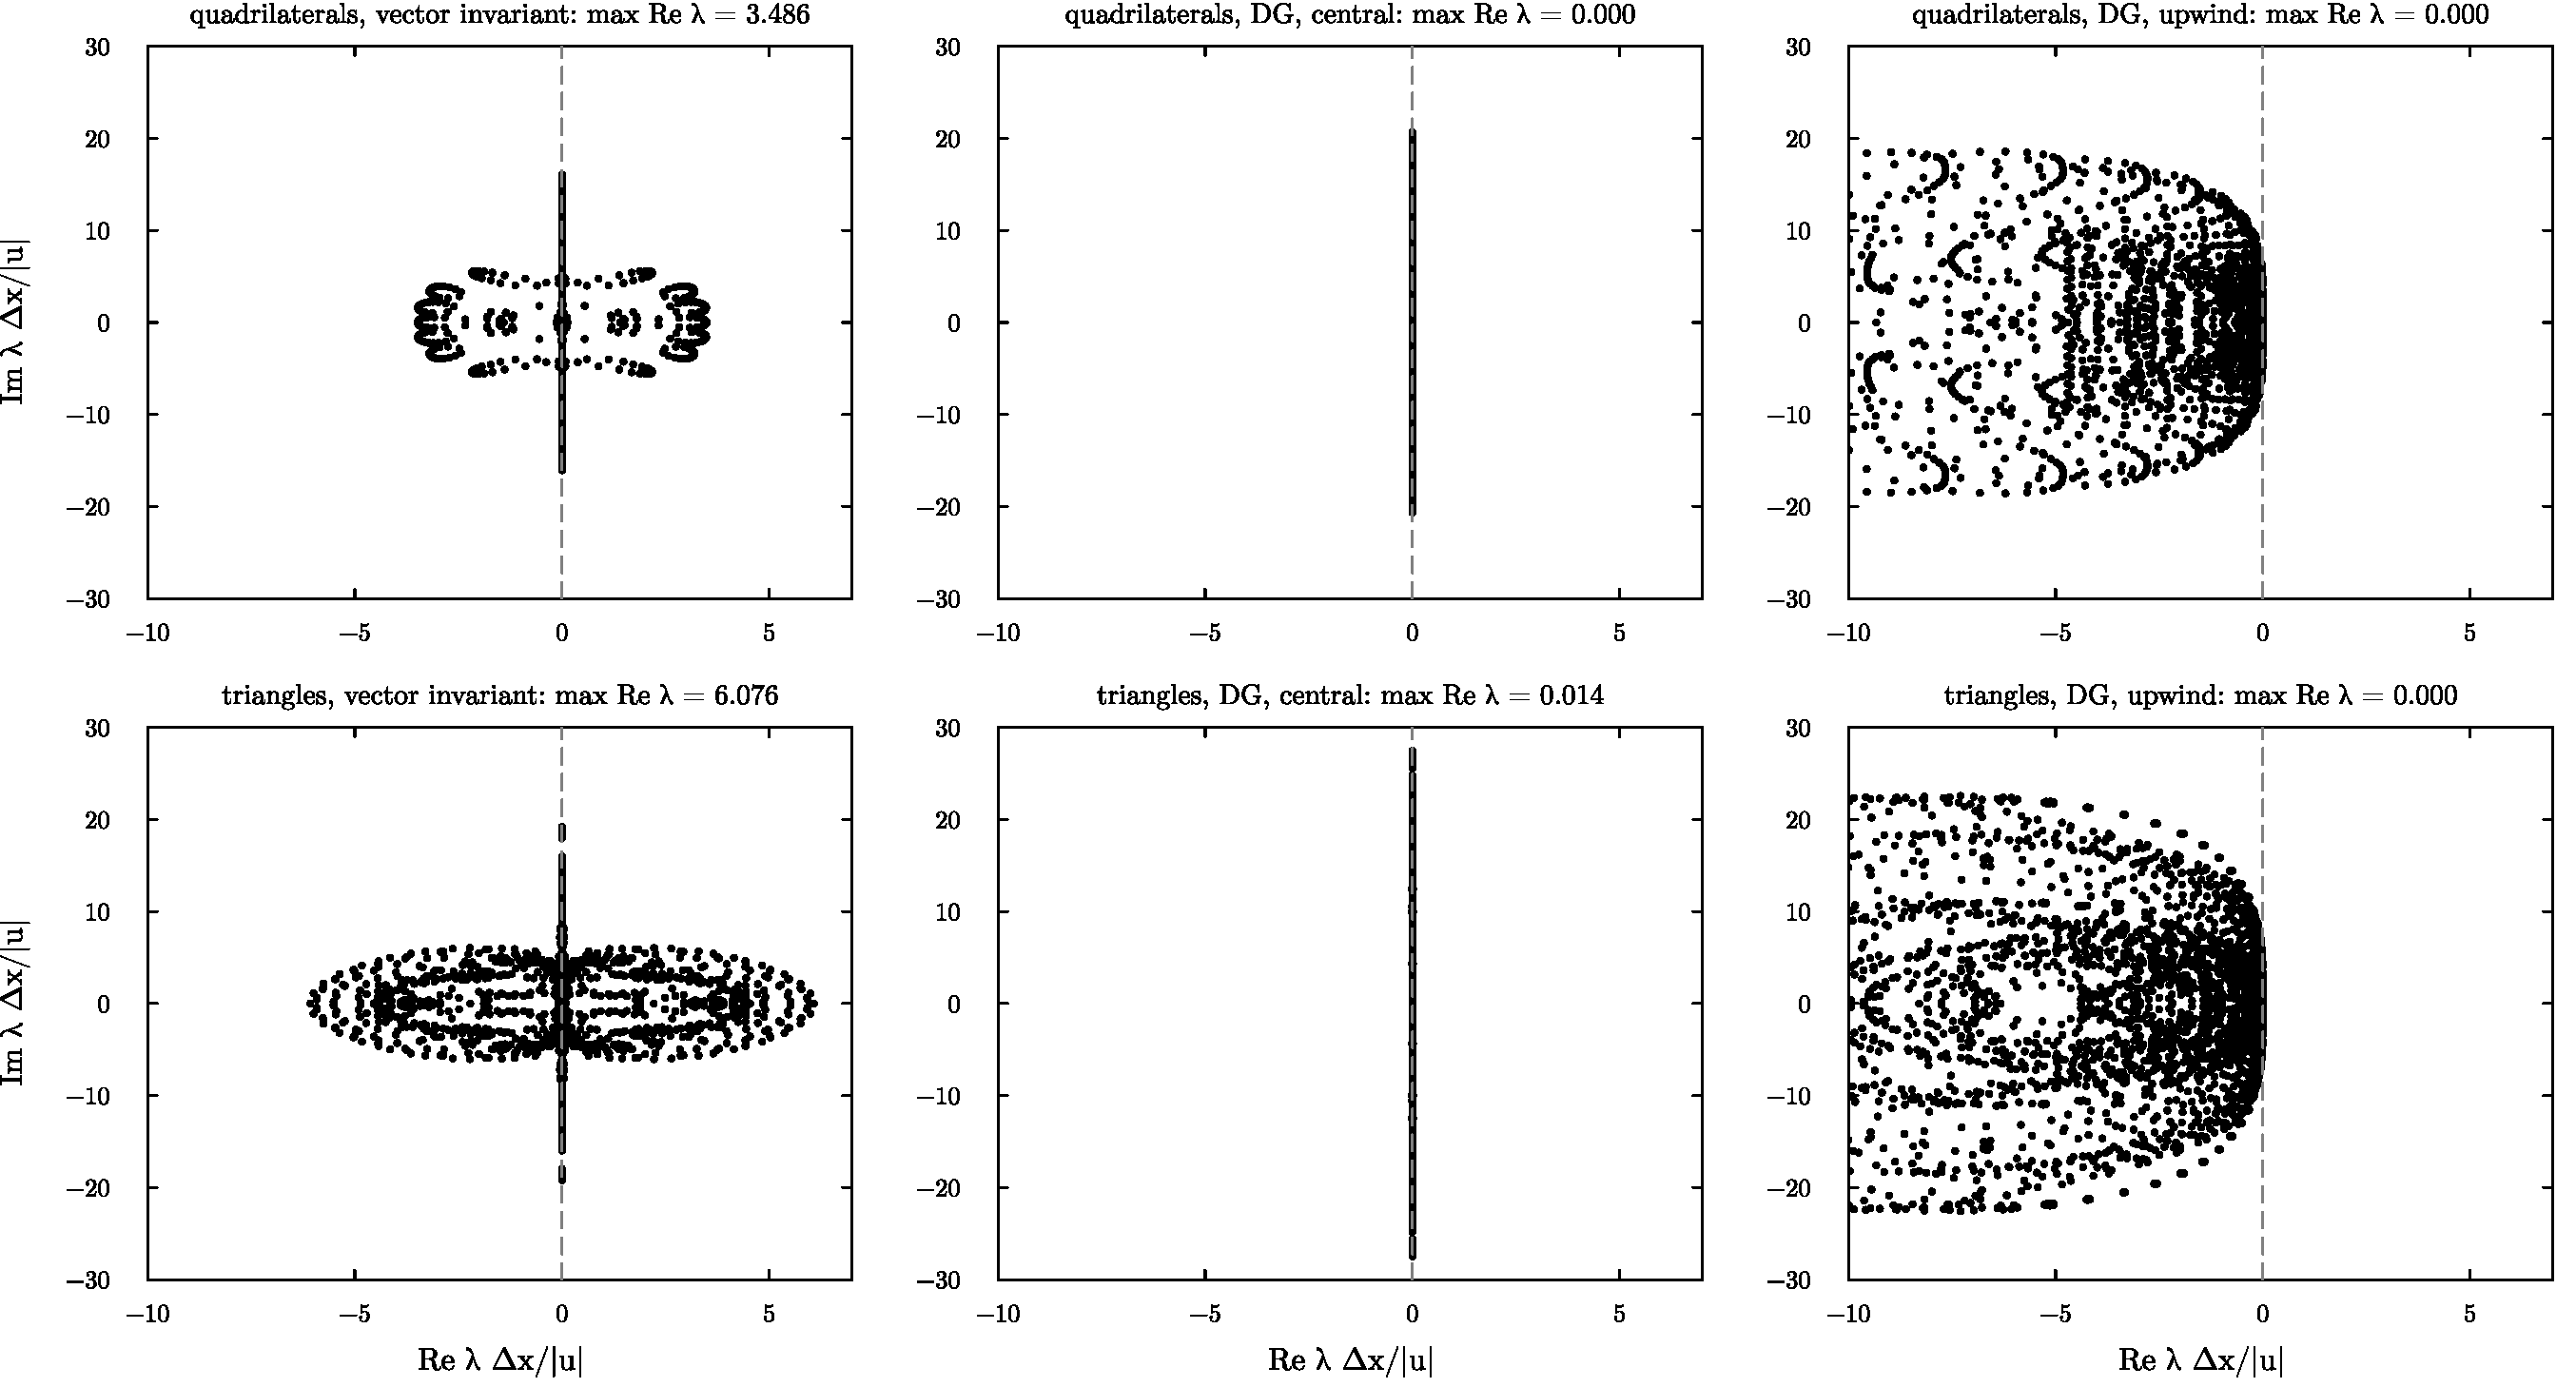
\includegraphics[width=\textwidth]{figures/kite_spectra.pdf}
\caption{Spectra of the linearized one-layer tendency in a uniform supercritical flow ($|\bu| = 1.04$, wave
speed $c = 0.5$, periodic $6\times6$ mesh), in units of $|\bu|/\Delta x$: vector-invariant form \eqref{eq:vi}
and DG form \eqref{eq:dg-theta}--\eqref{eq:dg-u} with central and upwind traces, on quadrilaterals (top) and
triangles (bottom).}
\label{fig:spectra}
\end{figure}

%==============================================================================
\section{Three-dimensional experiments}\label{sec:3d-results}
% TODO: all runs of this section were made with the previous vertical discretization; rerun them with the
% Galerkin vertical part of Section 7.4 and update the numbers and figures.

All runs use $\mathrm{RT}_1\times Q_2$ horizontally, 30 equidistant layers up to 30\,km, the absorbing layer
above 22\,km, the DG transport with upwind traces for $\theta$, $\rho$, $\bu$ and $w$, and no explicit
diffusion. They are serial CPU runs.

\subsection{Thermal wind}
A steady rotating wind in exact gradient-wind balance, $1/T = (1 + \varepsilon\sin^2\varphi\,
\mathrm{sech}^2(z/z_s))/T_0$ with $T_0 = 300$\,K, $\varepsilon = 0.1$, $z_s = 12$\,km and the same surface
pressure everywhere; the westerly reaches about 24\,m/s. A good model keeps it at rest in the rotating
frame (Figure~\ref{fig:thermal}). With the vector-invariant momentum, max\,$|w|$ grows on all meshes, to
$3\cdot10^{-2}$ (hexagons), 0.20 (cubed sphere) and NaN (triangles, day~2.5). With the DG momentum it stays
at about $10^{-4}$\,m/s on all three meshes, max $|\theta'|$ at $2\cdot10^{-2}$\,K and max $|\Delta p_s|$ at
$5\cdot10^{-2}$\,hPa.

\begin{figure}[t]
\centering
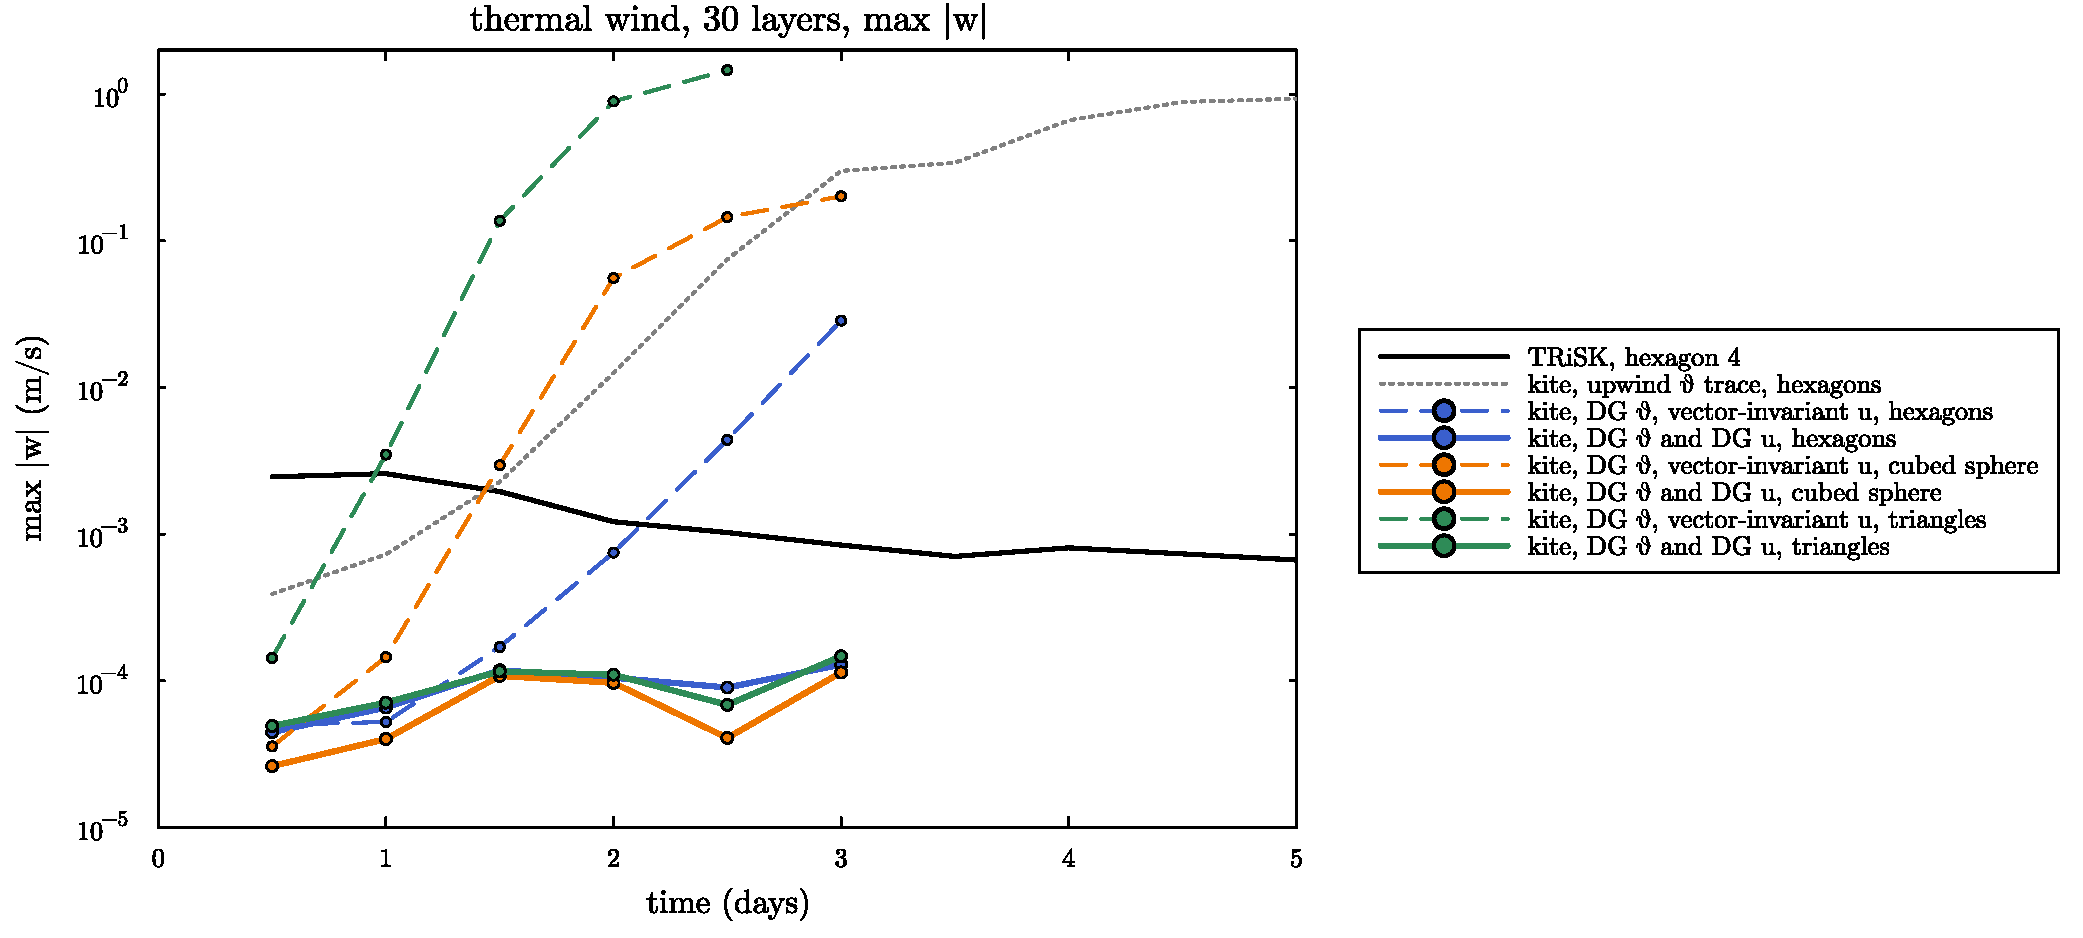
\includegraphics[width=\textwidth]{figures/kite3d_thermal_wind.pdf}
% TODO: regenerate without the reference curve of another model.
\caption{Thermal wind: max $|w|$ on hexagons 3 (23\,682 columns), the cubed sphere 12 (21\,600) and
triangles 3 (24\,320), with the upwind $\theta$ trace (grey), the DG $\theta$ transport with the
vector-invariant momentum (dashed) and the DG transport of $\theta$, $\rho$ and $\bu$ (solid).}
\label{fig:thermal}
\end{figure}

\subsection{Baroclinic wave in an $f$-plane channel}
The channel of Ullrich, Reed and Jablonowski \cite{Ullrich2015} is 40\,000\,km long and 6000\,km wide, with a
jet of 35\,m/s, $f_0 = 1.0313\cdot10^{-4}$\,s$^{-1}$, flat ground and a Gaussian perturbation of $u$
(1\,m/s, 600\,km). The kite model has no walls, so we use a doubly periodic box of twice the width with the
mirrored channel and the easterly jet; $v = 0$ at the walls then holds by symmetry, and the unperturbed state
is an exact steady state. For this setup linear quasi-geostrophic theory gives the most unstable wave at zonal
wavenumber 10 (4000\,km) with the growth rate $6.59\cdot10^{-6}$\,s$^{-1}$ \cite{Ullrich2015}.
Figure~\ref{fig:channel} shows the amplitude of this wave in the surface pressure on $60\times18$ cells
(667\,km), $\Delta t = 200$\,s. After an adjustment of two days it grows at
$5.9$--$6.6\cdot10^{-6}$\,s$^{-1}$, reaching $6.58\cdot10^{-6}$ at day~11, and saturates after day~12. The
triangles follow the quadrilaterals to plotting accuracy; with the vector-invariant momentum the triangle
run is dominated by a grid-scale mode from day~1. Figure~\ref{fig:channel-maps} shows the wave in the surface
pressure and the temperature at 500\,m. It grows as a packet downstream of the perturbation, and from day~12
the warm air is drawn into tongues that roll up by day~14 with a minimum surface pressure of 955.6\,hPa. On
the triangles the minima are within 0.7\,hPa (979.4\,hPa at day~12, 955.8\,hPa at day~14). From day~14 they
show small ripples in the temperature at the warm edge of the front.

\begin{figure}[t]
\centering
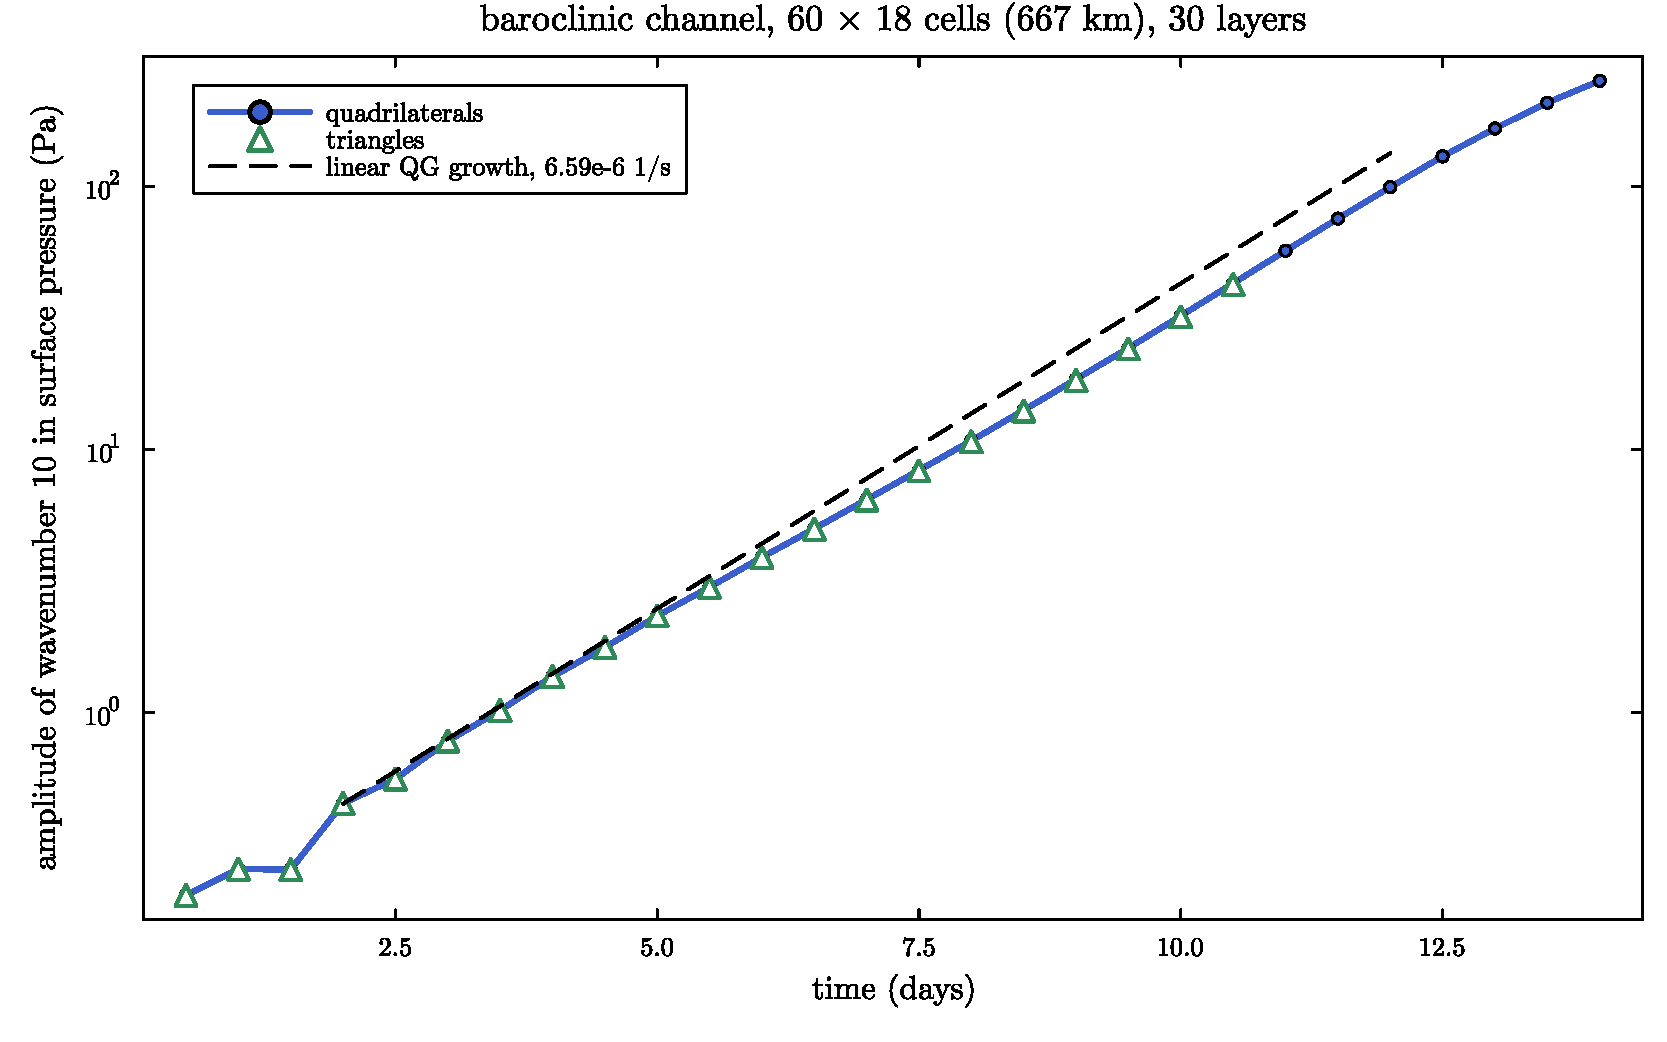
\includegraphics[width=0.8\textwidth]{figures/kite3d_channel_growth.pdf}
\caption{Baroclinic channel: amplitude of zonal wavenumber 10 of the surface pressure on $60\times18$
quadrilaterals (27\,000 columns) and triangles (41\,040 columns), and the growth rate of linear QG theory.}
\label{fig:channel}
\end{figure}

\begin{figure}[t]
\centering
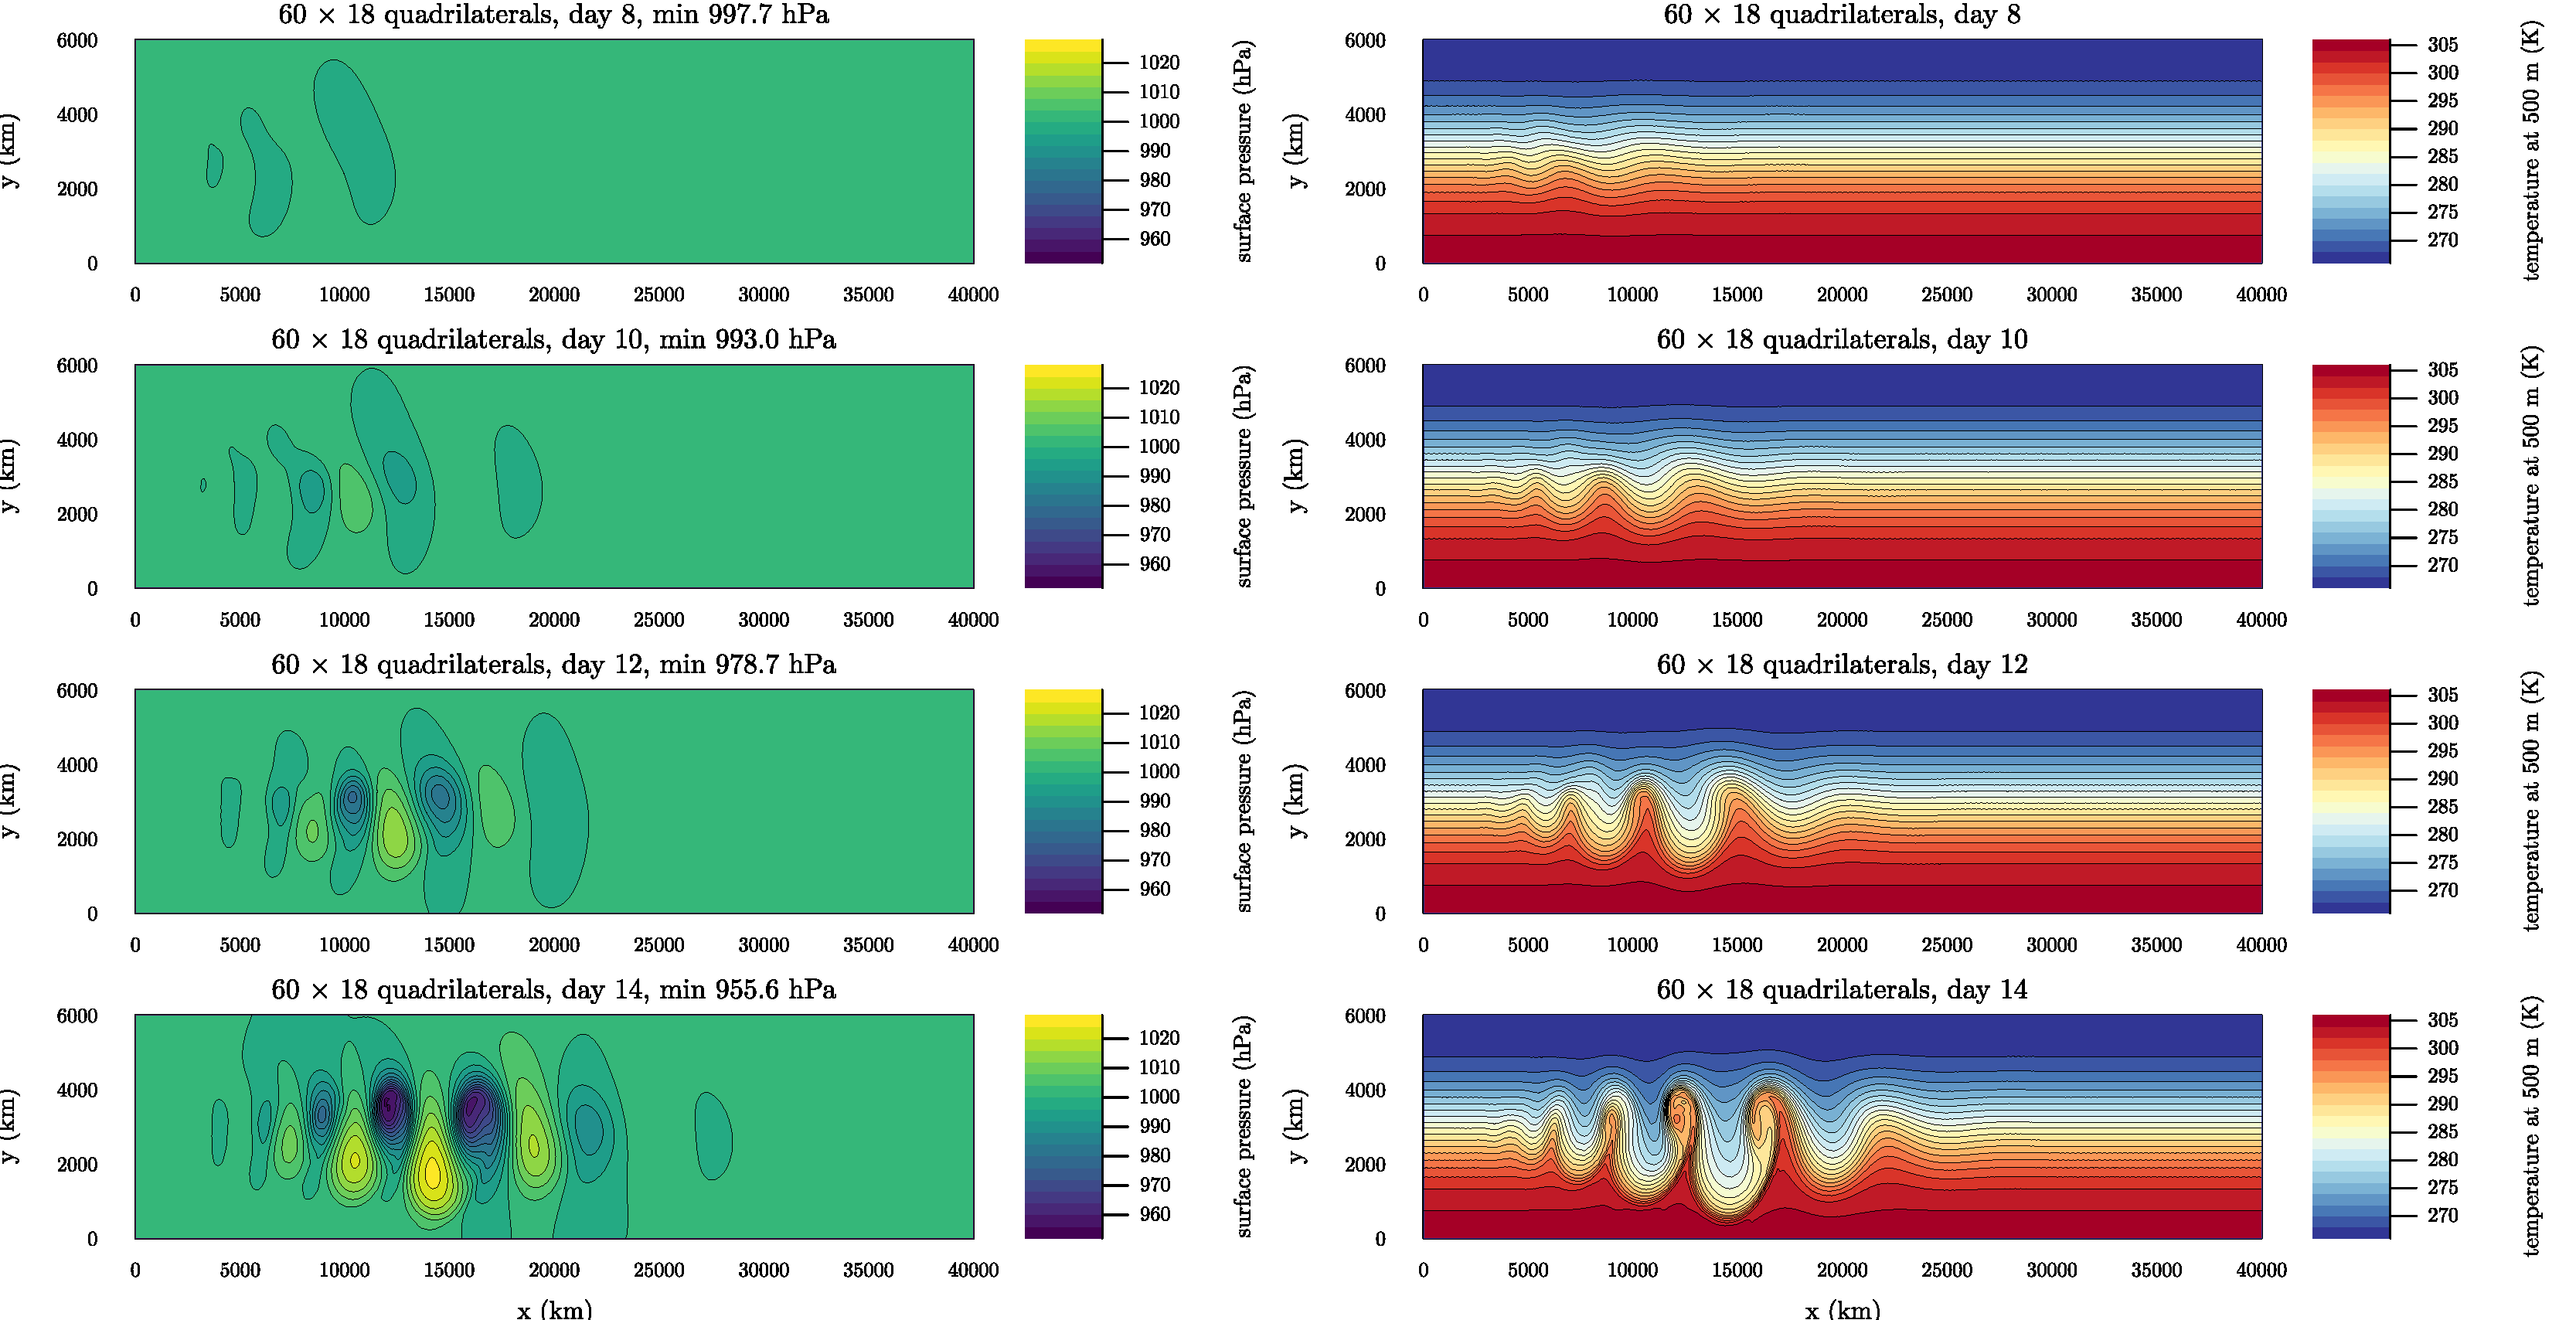
\includegraphics[width=\textwidth]{figures/kite3d_channel_quadrilateral.pdf}
\caption{Baroclinic channel on $60\times18$ quadrilaterals: surface pressure (left) and temperature at
500\,m (right) at days 8, 10, 12 and 14, the channel half $0 \le y \le 6000$\,km of the doubly periodic
box.}
\label{fig:channel-maps}
\end{figure}

\subsection{Baroclinic wave on the sphere}
The baroclinic wave of Ullrich et al.\ \cite{Ullrich2014} with the perturbation of DCMIP 2016, on hexagons 3,
the cubed sphere 12 and triangles 3 (about 23\,000 columns, roughly 130\,km between height nodes),
$\Delta t = 150$\,s. Minimum surface pressure (hPa):
\begin{center}
\begin{tabular}{lccccc}
\toprule
day & 6 & 7 & 8 & 9 & 10 \\
\midrule
hexagons (23\,682 columns) & 993.5 & 984.3 & 968.3 & 941.6 & 925.8 \\
cubed sphere (21\,600) & 993.4 & 984.1 & 966.9 & 942.7 & 926.3 \\
triangles (24\,320) & 993.4 & 984.7 & 967.3 & 936.0 & 925.4 \\
\bottomrule
\end{tabular}
\end{center}
The three meshes agree to 1\,hPa at day~10 (Figures~\ref{fig:bw-ps} and~\ref{fig:bw-T}); mass is conserved to $10^{-15}$. The maps show
the $Q_2$ fields evaluated inside the kites, not the nodal values. A lowest-order run ($Q_1$ heights) on
hexagon~3 reached only 976.6\,hPa, with max\,$|w|$ near 1\,m/s from grid-scale noise.

\begin{figure}[p]
\centering
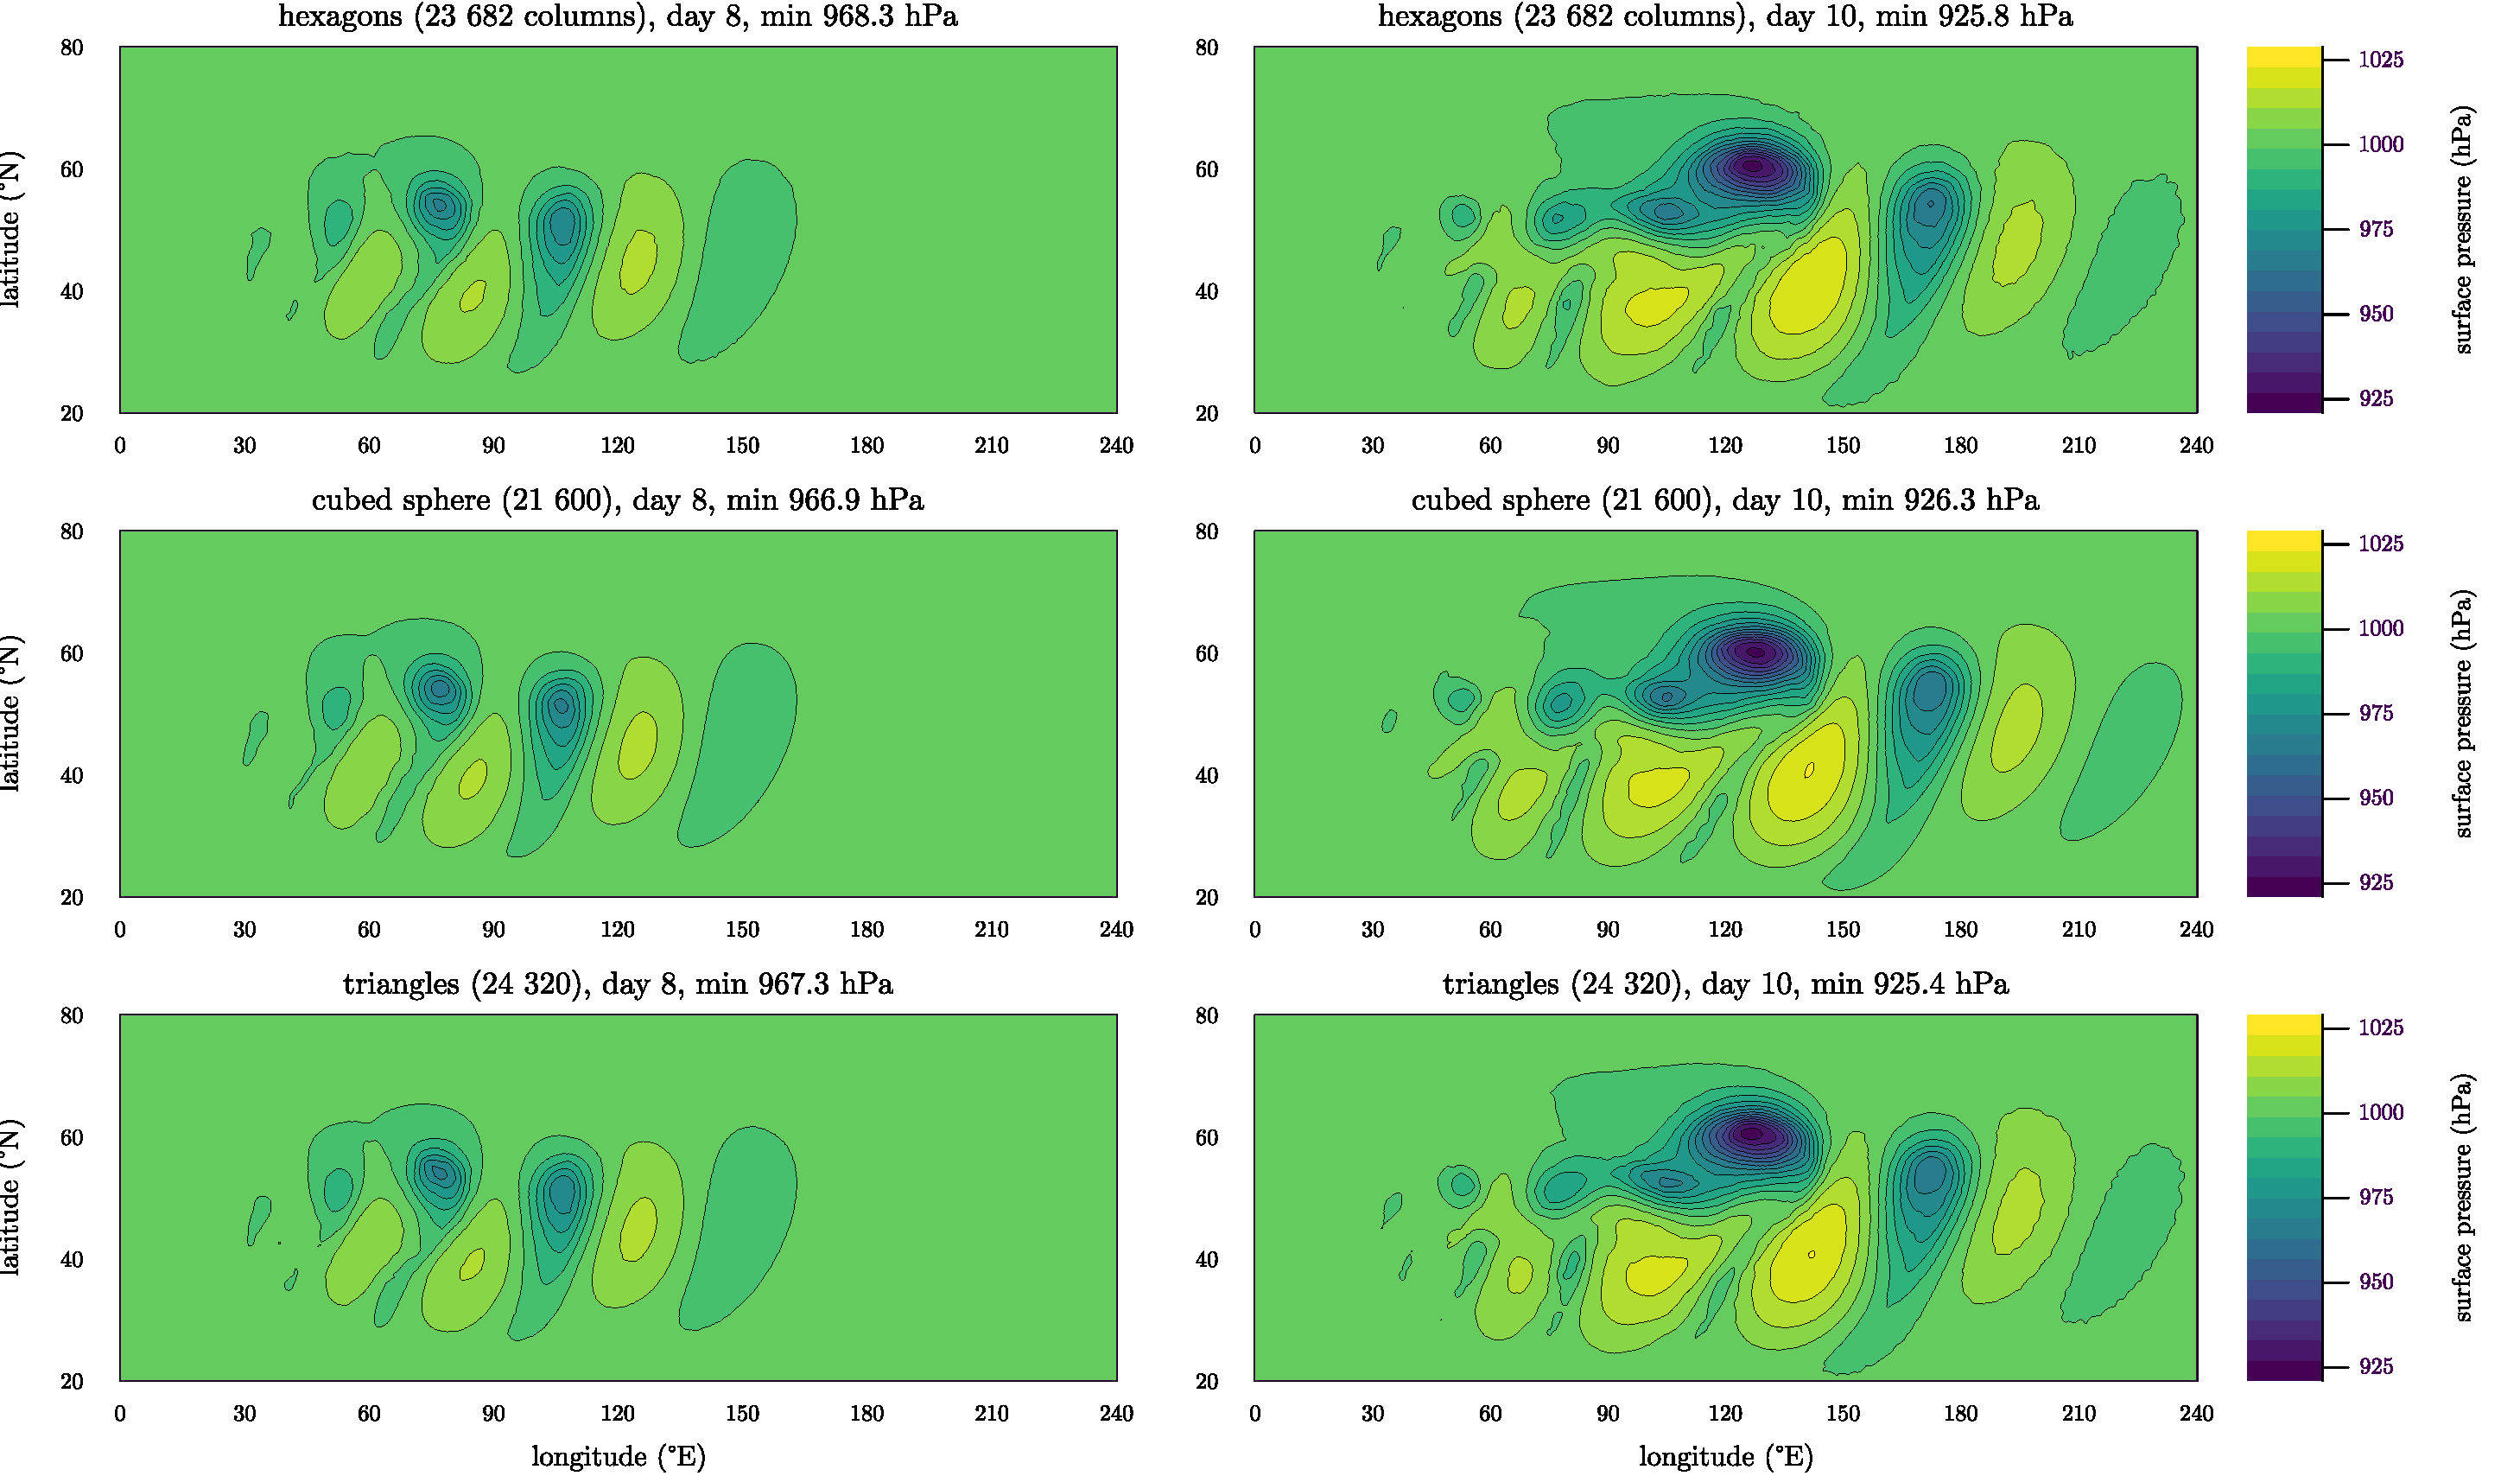
\includegraphics[width=\textwidth]{figures/kite3d_baroclinic_wave_ps.pdf}
\caption{Baroclinic wave, surface pressure at days 8 and 10 on the three kite meshes (contour interval
6\,hPa).}
\label{fig:bw-ps}
\end{figure}

\begin{figure}[p]
\centering
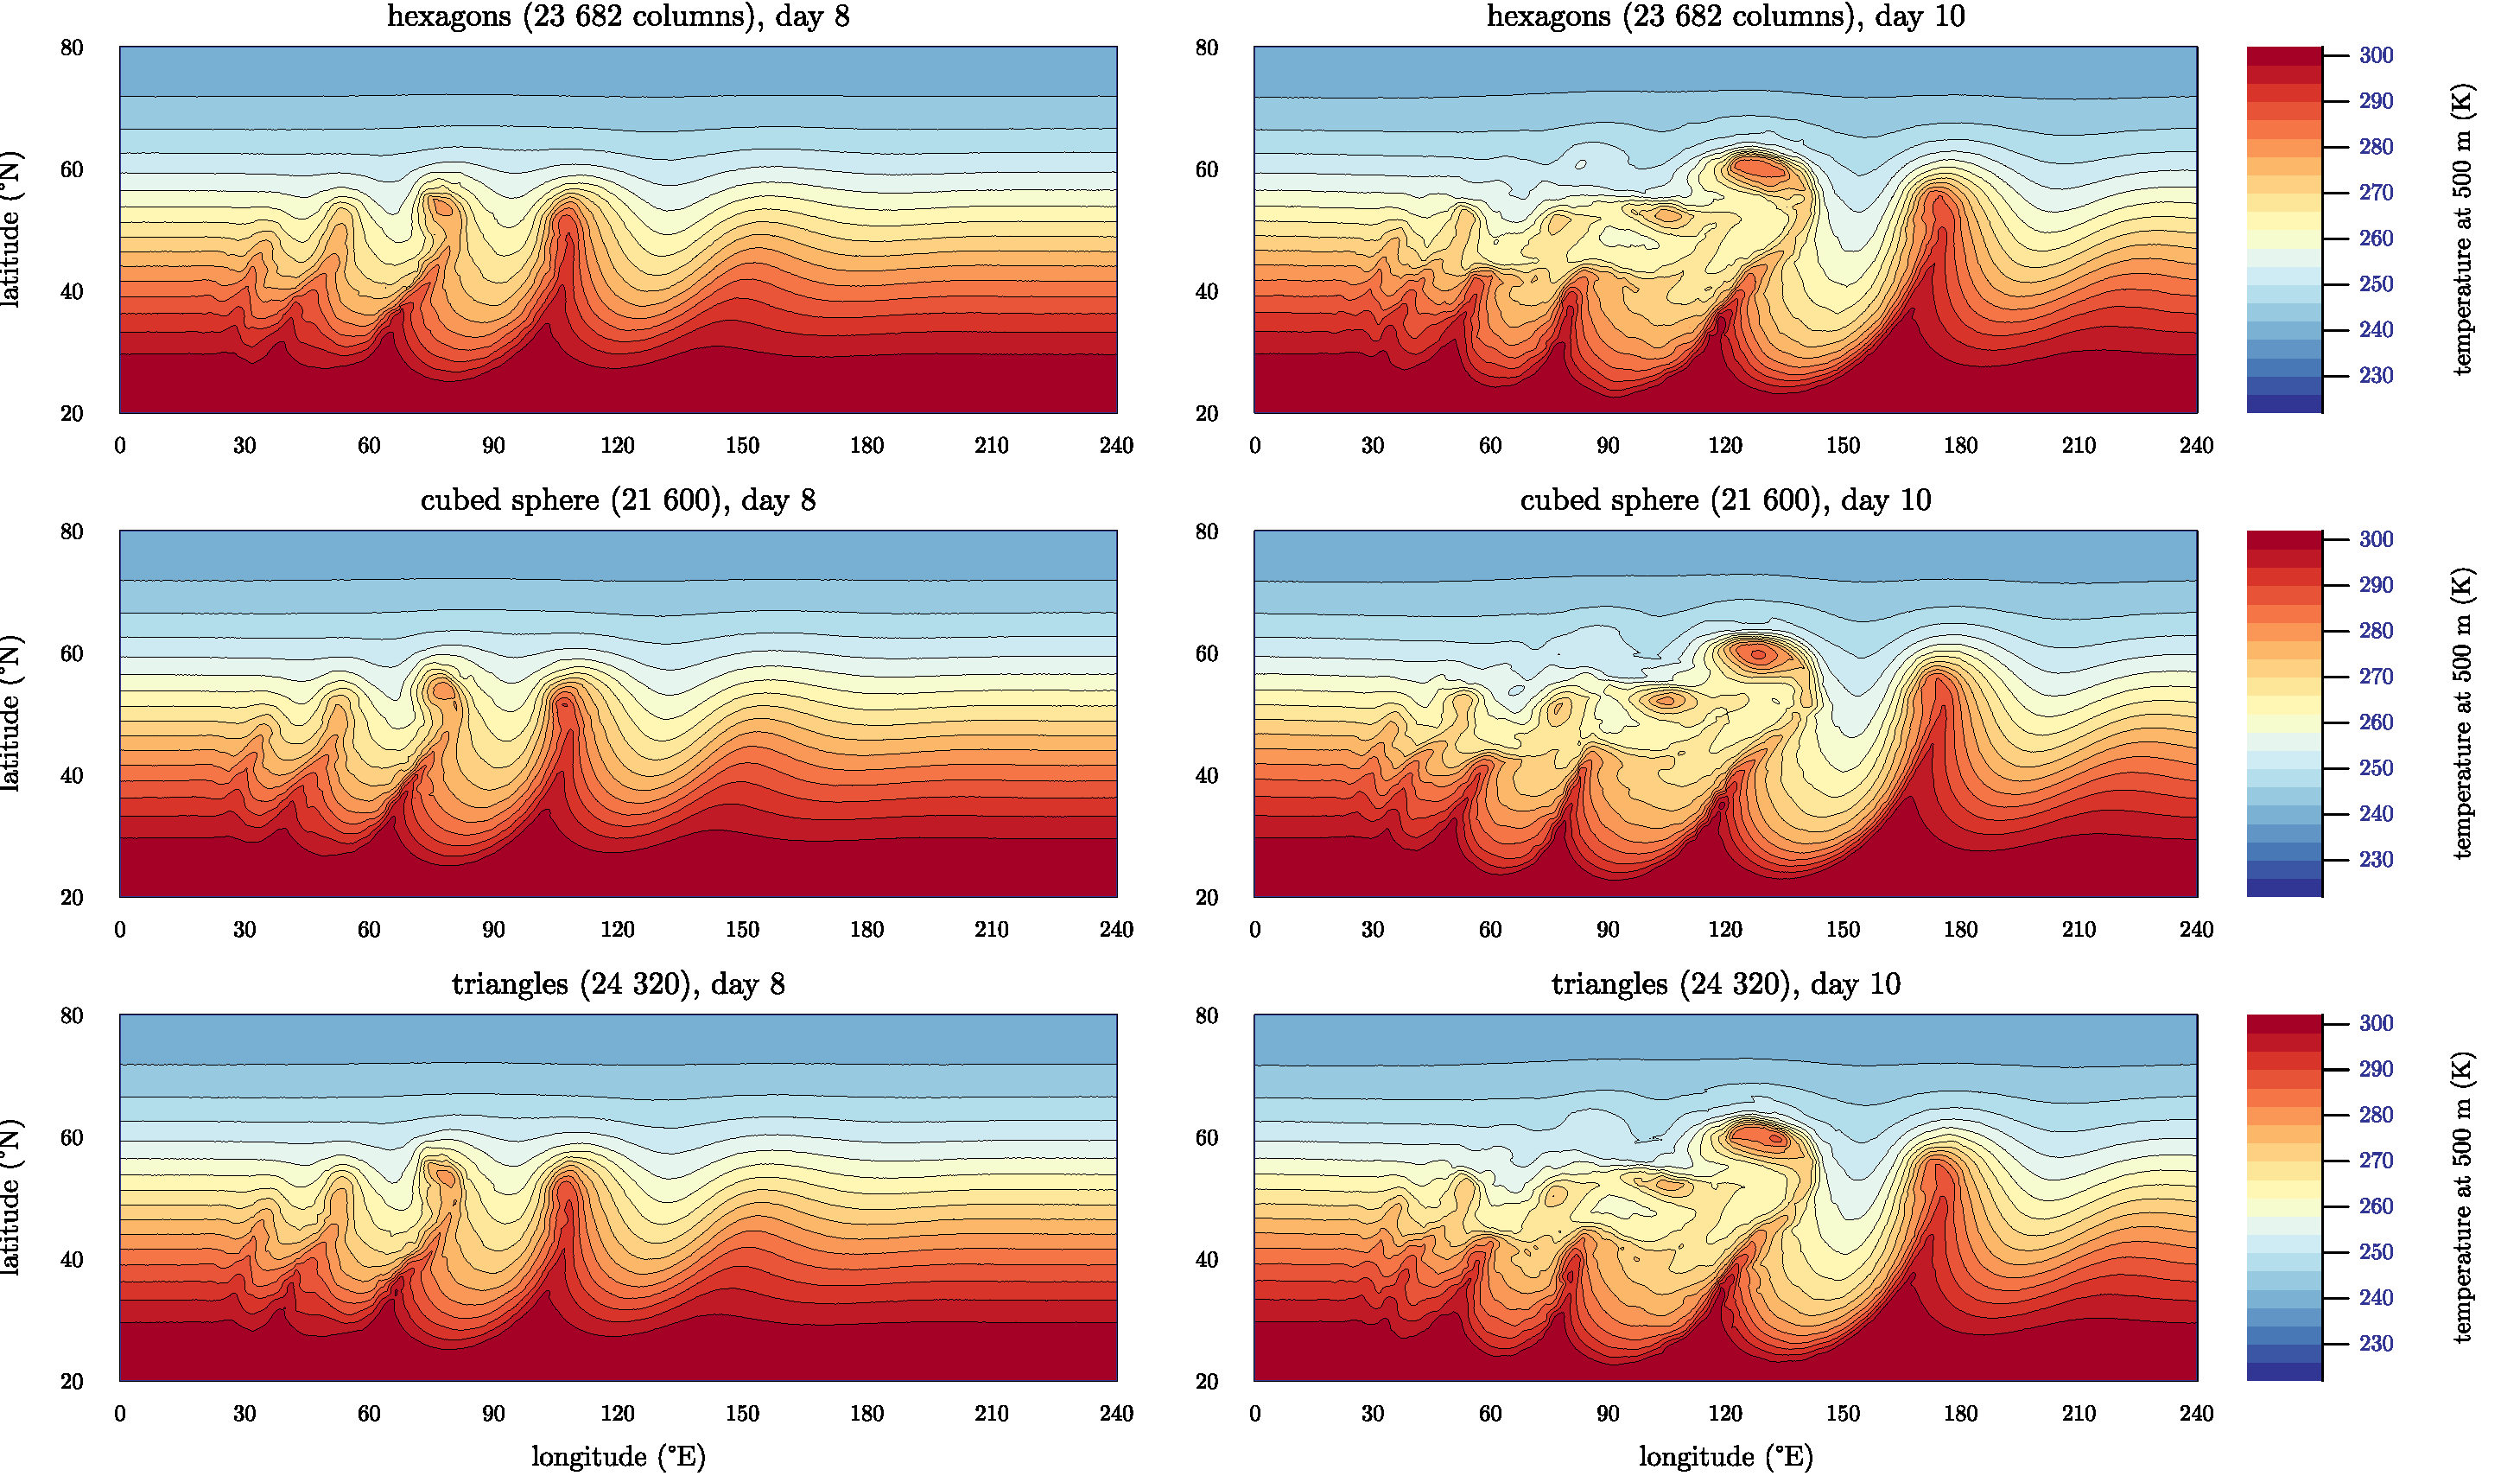
\includegraphics[width=\textwidth]{figures/kite3d_baroclinic_wave_T.pdf}
\caption{Baroclinic wave, temperature of the lowest layer (500\,m) at days 8 and 10 on the three kite
meshes (contour interval 4\,K).}
\label{fig:bw-T}
\end{figure}

%==============================================================================
\section{Related methods}\label{sec:related}

Table~\ref{tab:related} compares the kite method with the two closest ones. All three obtain local mass
matrices from a staggered pair of macro-element meshes.

\begin{table}[t]
\centering
\caption{The kite method and the two closest staggered methods.}
\label{tab:related}
\footnotesize
\begin{tabular}{p{1.6cm}p{3.4cm}p{3.4cm}p{3.6cm}}
\toprule
& Wess et al.\ \cite{Wess2024} & Leng, Lan, Ju \cite{LengLanJu2026} & kite method \\
\midrule
mesh & triangles, barycentric dual cells around the vertices &
  polygons split into triangles around an interior point; dual elements: the two triangles of an edge &
  polygons split into kites; dual cells around the vertices, orthogonal dual where it exists \\
continuity & one field conforming on the primal mesh, the other in the dual cells &
  velocity normal-continuous in the polygons, height continuous in the edge pairs &
  height continuous in the polygons, velocity normal-continuous in the dual cells \\
spaces & lumped $Q_p$ scalars and $Q_p\times Q_p$ vectors, any $p$ &
  BDM$_1$ velocity, $P_1$ height & $\mathrm{RT}_k$ velocity, $Q_{k+1}$ Radau heights (BDM and the pair of
  \cite{Wess2024} as options) \\
mass matrices & diagonal / small blocks & block diagonal & diagonal height, dual-cell velocity blocks \\
geometry & plane & sphere, curved triangles & sphere, curved kites, metric-free Piola \\
equations & acoustics, Maxwell & nonlinear shallow water & nonlinear shallow water, compressible Euler \\
\bottomrule
\end{tabular}
\end{table}

The equal-order pairs (the pair of \cite{Wess2024}, the BDM$_1\times P_1$ pair of \cite{LengLanJu2026})
have no spurious pressure modes; for the kite pair $\mathrm{RT}_k\times Q_{k+1}$ the velocity splits exactly
into gradients and curls, and the price is the $N$ stationary height modes of Theorem~\ref{thm:kernel}.
The vertical part of the kite model is the lowest-order compatible extruded pair
\cite{NataleShiptonCotter2016,Melvin2019}, but with the trapezoidal rule in place of exact integration, so that
the vertical mass is diagonal and the columns at the Radau nodes decouple; its formulas coincide with those of
a Lorenz-staggered finite-volume column. The C-grid finite-volume models \cite{Thuburn2009,Ringler2010,Zaengl2015}
have the same mass and energy properties at first order on general meshes.

%==============================================================================
\section{Conclusions}\label{sec:conclusions}

The kite spaces give staggered finite elements on arbitrary polygonal meshes with diagonal height and
block-diagonal velocity mass matrices. For $\mathrm{RT}_k\times Q_{k+1}$ the velocity space splits exactly
into discrete gradients and curls, with one stationary height mode per primal cell. In shallow water the
scheme conserves mass and energy exactly, converges at second order on hexagonal, triangular and
quadrilateral meshes and runs on GPUs and with MPI. The vertical part, derived as a Galerkin method with the
trapezoidal rule, keeps the column structure of HEVI schemes and exchanges energy exactly. The horizontal
transport must be built with care in three dimensions: the velocity mass must use the rule of the projections,
scalars must be transported by DG, and in supercritical flow, which the higher vertical modes of a stratified
atmosphere always are, the energy-conserving vector-invariant momentum transport is unstable. A DG transport
of momentum and density with the pointwise velocity and upwind traces removes this instability on all
meshes. With it the model is quiet on the thermal wind, reproduces the linear baroclinic growth rate in a
channel and gives the same baroclinic wave on three different meshes.

Open points: the DG momentum form is not energy conserving, because the kinetic energy of the advective form
differs from the projected $K$ of the pressure term; whether an energy-conserving skew-symmetric form with the
same stability exists is open. The sub-cell height modes are seen by the vertical but not by the horizontal
pressure gradient; a pair without them, or a filter of the modes, is to be tested in 3D. The DG terms are
serial CPU loops so far. Charney--Phillips staggering, with $\theta$ in the space of $w$, and higher vertical
order are the next steps for the vertical part. Orography needs the thickness-weighted velocity mass of Section~\ref{sec:orography}; a
separable terrain-following coordinate or the static condensation of the kite blocks keeps its cost low.

\section*{Code availability}
{\sloppy
\code{dmplex.jl} (\url{https://github.com/OsKnoth/dmplex}), the models \code{NonlinearKiteShallowWater} and
\code{KiteNonhydrostatic}. The examples \code{galewsky.jl}, \code{bickley.jl}, \code{thermal\_wind.jl} and
\code{baroclinic\_channel.jl} run the test cases; the figure scripts are in \code{docs/paper/scripts}.\par}

%==============================================================================
\begin{thebibliography}{99}
\bibitem{ArakawaMoorthi1988} A.~Arakawa and S.~Moorthi, Baroclinic instability in vertically discrete systems,
  \emph{J. Atmos. Sci.} 45 (1988) 1688--1707.
\bibitem{ChungEngquist2006} E.~T. Chung and B.~Engquist, Optimal discontinuous Galerkin methods for wave
  propagation, \emph{SIAM J. Numer. Anal.} 44 (2006) 2131--2158.
\bibitem{ChungLamQian2015} E.~T. Chung, C.~Y. Lam and J.~Qian, A staggered discontinuous Galerkin method for
  the simulation of seismic waves with surface topography, \emph{Geophysics} 80 (2015) T119--T135.
  % TODO: check volume and pages
\bibitem{CotterShipton2012} C.~J. Cotter and J.~Shipton, Mixed finite elements for numerical weather
  prediction, \emph{J. Comput. Phys.} 231 (2012) 7076--7091.
\bibitem{DuChung2021} J.~Du and E.~Chung, Mortar DG method with staggered hybridization for Rayleigh waves
  simulation, \emph{Commun. Comput. Phys.} 29 (2021) 111--127.
\bibitem{Galewsky2004} J.~Galewsky, R.~K. Scott and L.~M. Polvani, An initial-value problem for testing
  numerical models of the global shallow-water equations, \emph{Tellus A} 56 (2004) 429--440.
\bibitem{Klemp2008} J.~B. Klemp, J.~Dudhia and A.~D. Hassiotis, An upper gravity-wave absorbing layer for NWP
  applications, \emph{Mon. Wea. Rev.} 136 (2008) 3987--4004.
\bibitem{LengLanJu2026} W.~Leng, R.~Lan and L.~Ju, A conservative staggered discontinuous Galerkin method on
  triangular grids for the shallow water equations, \emph{J. Comput. Phys.} 546 (2026) 114503.
\bibitem{McRaeCotter2014} A.~T.~T. McRae and C.~J. Cotter, Energy- and enstrophy-conserving schemes for
  the shallow-water equations, based on mimetic finite elements, \emph{Q. J. R. Meteorol. Soc.} 140 (2014)
  2223--2234.
\bibitem{Melvin2019} T.~Melvin, T.~Benacchio, B.~Shipway, N.~Wood, J.~Thuburn and C.~Cotter, A mixed
  finite-element, finite-volume, semi-implicit discretization for atmospheric dynamics: Cartesian geometry,
  \emph{Q. J. R. Meteorol. Soc.} 145 (2019) 2835--2853.
\bibitem{NataleShiptonCotter2016} A.~Natale, J.~Shipton and C.~J. Cotter, Compatible finite element spaces
  for geophysical fluid dynamics, \emph{Dyn. Stat. Clim. Syst.} 1 (2016) dzw005.
\bibitem{Ringler2010} T.~D. Ringler, J.~Thuburn, J.~B. Klemp and W.~C. Skamarock, A unified approach to
  energy conservation and potential vorticity dynamics for arbitrarily-structured C-grids,
  \emph{J. Comput. Phys.} 229 (2010) 3065--3090.
\bibitem{Thuburn2009} J.~Thuburn, T.~D. Ringler, W.~C. Skamarock and J.~B. Klemp, Numerical representation
  of geostrophic modes on arbitrarily structured C-grids, \emph{J. Comput. Phys.} 228 (2009) 8321--8335.
\bibitem{ThuburnWoollings2005} J.~Thuburn and T.~J. Woollings, Vertical discretizations for compressible Euler
  equation atmospheric models giving optimal representation of normal modes, \emph{J. Comput. Phys.} 203
  (2005) 386--404.
\bibitem{Ullrich2014} P.~A. Ullrich, T.~Melvin, C.~Jablonowski and A.~Staniforth, A proposed baroclinic wave
  test case for deep- and shallow-atmosphere dynamical cores, \emph{Q. J. R. Meteorol. Soc.} 140 (2014)
  1590--1602.
\bibitem{Ullrich2015} P.~A. Ullrich, K.~A. Reed and C.~Jablonowski, Analytical initial conditions and an
  analysis of baroclinic instability waves in $f$- and $\beta$-plane 3D channel models,
  \emph{Q. J. R. Meteorol. Soc.} 141 (2015) 2972--2988.
\bibitem{Abdelfattah2017} A.~Abdelfattah, A.~Haidar, S.~Tomov and J.~Dongarra, Fast Cholesky factorization on
GPUs for batch and native modes in MAGMA, J. Comput. Sci. 20 (2017) 85--93.

\bibitem{Wess2024} M.~Wess, B.~Kapidani, L.~Codecasa and J.~Sch\"oberl, Mass lumping the dual cell method to
  arbitrary polynomial degree for acoustic and electromagnetic waves, \emph{J. Comput. Phys.} 513 (2024)
  113196.
\bibitem{WickerSkamarock2002} L.~J. Wicker and W.~C. Skamarock, Time-splitting methods for elastic models
  using forward time schemes, \emph{Mon. Wea. Rev.} 130 (2002) 2088--2097.
\bibitem{White2005} A.~A. White, B.~J. Hoskins, I.~Roulstone and A.~Staniforth, Consistent approximate models
  of the global atmosphere: shallow, deep, hydrostatic, quasi-hydrostatic and non-hydrostatic,
  \emph{Q. J. R. Meteorol. Soc.} 131 (2005) 2081--2107.
\bibitem{Williamson1992} D.~L. Williamson, J.~B. Drake, J.~J. Hack, R.~Jakob and P.~N. Swarztrauber, A standard
  test set for numerical approximations to the shallow water equations in spherical geometry,
  \emph{J. Comput. Phys.} 102 (1992) 211--224.
\bibitem{Zaengl2015} G.~Z\"angl, D.~Reinert, P.~R\'ipodas and M.~Baldauf, The ICON (ICOsahedral
  Non-hydrostatic) modelling framework of DWD and MPI-M: description of the non-hydrostatic dynamical core,
  \emph{Q. J. R. Meteorol. Soc.} 141 (2015) 563--579.
\bibitem{GalChen1975} T.~Gal-Chen and R.~C.~J. Somerville, On the use of a coordinate transformation for the
  solution of the Navier--Stokes equations, \emph{J. Comput. Phys.} 17 (1975) 209--228.
\bibitem{Schaer2002} C.~Sch\"ar, D.~Leuenberger, O.~Fuhrer, D.~L\"uthi and C.~Girard, A new terrain-following
  vertical coordinate formulation for atmospheric prediction models, \emph{Mon. Wea. Rev.} 130 (2002)
  2459--2480.
\end{thebibliography}

\end{document}
